% ===========================================================================
% GridSpike -- SUPPLEMENTARY MATERIAL (anonymized), companion to main.tex.
% Standalone elsarticle document in review style; section, table, figure and
% equation numbers carry an S prefix and are referenced from the manuscript
% through the xr package (\externaldocument), so both builds share labels.
% Build:  pdflatex supplementary && bibtex supplementary && pdflatex x2
%         (build BEFORE main.tex so that main.aux can pull the S-labels;
%          this file in turn resolves manuscript labels through main.aux)
% ===========================================================================
\documentclass[review,12pt]{elsarticle}

\usepackage[T1]{fontenc}
\usepackage[utf8]{inputenc}
\usepackage{amsmath,amssymb}
\usepackage{graphicx}
\usepackage[dvipsnames]{xcolor}
\usepackage{booktabs}
\usepackage{array}
\usepackage{multirow}
\usepackage{tabularx}
\usepackage{rotating}
% landscape pages that also open rotated in PDF viewers (wide tables S1 and S21)
\usepackage{pdflscape}
\usepackage{algorithm}
\usepackage{algpseudocode}
\usepackage[hidelinks]{hyperref}
\usepackage{xr}
\externaldocument{main}

% ---------------------------------------------------------------------------
% macros.tex -- shared macros for the manuscript.
%
% The cardinal rule of this project: NO FABRICATED NUMBERS. Every numeric result
% must come from a generated file. Until the experiment battery lands, every
% place where a number belongs carries \TODOnum{...}, which typesets a loud red
% marker that cannot be mistaken for a value in a compiled PDF.
% ---------------------------------------------------------------------------

% \TODOnum{label} -- a results-shaped hole. The argument is a short tag naming
% what belongs there, so the battery-to-manuscript wiring is unambiguous.
% \TODOnum{} (empty argument) is the bare marker.
\newcommand{\TODOnum}[1]{%
  \textcolor[rgb]{0.85,0.0,0.0}{\textbf{[\,??\,\ifx\relax#1\relax\else\,\textsf{\footnotesize #1}\,\fi]}}%
}

% \TODOfig{filename}{what the figure will show} -- a placeholder frame for a
% figure that only the battery can produce. Never an \includegraphics of a
% missing file, so the document always compiles and the hole is loud.
\newcommand{\TODOfig}[2]{%
  \begingroup
  \setlength{\fboxrule}{1.2pt}%
  \setlength{\fboxsep}{10pt}%
  \textcolor[rgb]{0.85,0.0,0.0}{%
    \fbox{\parbox[c][7.5\baselineskip][c]{0.86\linewidth}{\centering
      \textbf{FIGURE PENDING}\\[4pt]
      \texttt{figures/#1}\\[6pt]
      \normalfont\itshape #2}}}%
  \endgroup
}

% Short-hand for the system name, so a rename is a one-line edit.
\newcommand{\sysname}{GridSpike}

% Units / symbols used repeatedly.
\newcommand{\uJ}{\ensuremath{\mu\mathrm{J}}}
\newcommand{\pJ}{\ensuremath{\mathrm{pJ}}}
\newcommand{\ms}{\ensuremath{\mathrm{ms}}}
\newcommand{\macroF}{macro-F\textsubscript{1}}
\newcommand{\SynOps}{SynOps}

% Event-class names, typeset consistently.
\newcommand{\cls}[1]{\textsc{\small #1}}

% Table template shared by every table (generated and hand-written):
% tabularx at \linewidth, \scriptsize, \arraystretch 1.15, booktabs rules,
% caption above, notes in \tablenota below the rule.
\newcolumntype{L}{>{\raggedright\arraybackslash}X}
\newcolumntype{C}{>{\centering\arraybackslash}X}
% Y{r}: ragged X column at r times the average X width (ratios sum to the X count).
\newcolumntype{Y}[1]{>{\raggedright\arraybackslash\hsize=#1\hsize}X}
\newcommand{\tablenota}[1]{\par\smallskip\begin{minipage}{\linewidth}\scriptsize #1\end{minipage}}


% --- S numbering for every counter the manuscript may reference -------------
\renewcommand{\thepage}{S\arabic{page}}
\renewcommand{\thesection}{S\arabic{section}}
\renewcommand{\thesubsection}{S\arabic{section}.\arabic{subsection}}
\renewcommand{\thetable}{S\arabic{table}}
\renewcommand{\thefigure}{S\arabic{figure}}
\renewcommand{\theequation}{S\arabic{equation}}

\journal{Engineering Applications of Artificial Intelligence}

\begin{document}

\begin{frontmatter}

\title{Supplementary material for \emph{\sysname}: defense-aware
stress-testing of federated edge intelligence for event classification in
IEC 61850 substations}

\begin{abstract}
This document carries the material that the page budget of the main
manuscript could not hold: the formal notation and the equations the body
summarizes (Section~\ref{sec:sup-prelim}), the extended related-work
discussion and the positioning table (Section~\ref{sec:sup-related}), the
full benchmark-realism parameter audit and the generated-federation
inventory (Section~\ref{sec:sup-testbed}), the battery, provenance and
pre-registration detail (Section~\ref{sec:sup-design}), and the complete
set of secondary results tables, the full statistical battery and the
auxiliary figures (Section~\ref{sec:sup-results}). Nothing in it revises a
number in the manuscript; every table is generated by the same analysis
code from the same merged run corpus.
\end{abstract}

\end{frontmatter}

\section{Notation and formal definitions}
\label{sec:sup-prelim}

This section states the notation the manuscript compresses into prose.

\subsection{Cross-silo federated learning}
\label{sec:sup-fl}

Let $K$ substations hold private datasets $\mathcal{D}_1,\dots,\mathcal{D}_K$
with $n_k = |\mathcal{D}_k|$ and $n=\sum_k n_k$. Federated learning minimizes
the weighted empirical risk
\begin{equation}
\begin{aligned}
\min_{w}\; F(w) &\;=\; \sum_{k=1}^{K} \frac{n_k}{n}\, F_k(w), \\[2pt]
F_k(w) &\;=\; \frac{1}{n_k}\!\!\sum_{(x,y)\in\mathcal{D}_k}\!\! \ell\!\left(f_w(x), y\right),
\end{aligned}
\label{eq:fedobj}
\end{equation}
without moving $\mathcal{D}_k$. In FedAvg \cite{mcmahan2017} the server
broadcasts $w^{(t)}$, each client runs $E$ local epochs to obtain
$w_k^{(t+1)}$ and the server aggregates
$w^{(t+1)} = \sum_k (n_k/n)\, w_k^{(t+1)}$. FedProx \cite{li2020fedprox}
adds a proximal term to the \emph{client} objective,
\begin{equation}
\tilde{F}_k(w) \;=\; F_k(w) \;+\; \frac{\mu}{2}\bigl\lVert w - w^{(t)}\bigr\rVert_2^2 ,
\label{eq:fedprox}
\end{equation}
which limits client drift under heterogeneity and reduces to FedAvg at
$\mu=0$. Throughout, $\Delta_k = w_k - w^{(t)}$ is the \emph{update
direction} of client $k$ in a round: clients exchange full parameter
vectors, but every defense operates on $\Delta_k$, because full vectors
are dominated by the shared global component and are nearly collinear.

\subsection{Spiking neurons, coding and SynOps accounting}
\label{sec:sup-snn}

\paragraph{Neuron model}
The spiking classifier uses hard-reset leaky integrate-and-fire (LIF)
neurons unrolled over $T$ internal timesteps. For a layer of $n$ neurons
with input current $I_t$,
\begin{equation}
\begin{aligned}
u_t &= \beta \odot u_{t-1} + I_t, \qquad
s_t = H\!\left(u_t - \vartheta\right), \\[2pt]
u_t &\leftarrow u_t \odot \left(1 - \mathrm{sg}[s_t]\right),
\end{aligned}
\label{eq:lif}
\end{equation}
where $H$ is the Heaviside step, $\mathrm{sg}[\cdot]$ is the stop-gradient
operator (the reset carries no gradient), and both the decay
$\beta\in(0,1)^n$ and the threshold $\vartheta\in\mathbb{R}^n$ are learned
per neuron. The non-differentiable step is trained with the arctangent
surrogate gradient
\begin{equation}
\frac{\partial \tilde{s}}{\partial v} \;=\; \frac{\alpha/2}{1 + \left(\tfrac{\pi \alpha v}{2}\right)^2},
\qquad v = u_t - \vartheta,\; \alpha = 2 ,
\label{eq:surrogate}
\end{equation}
the documented default recipe of the reference toolkit
\cite{eshraghian2023,fang2023spikingjelly}. Logits are rate-decoded: the
linear readout is accumulated over the unroll and divided by $T$.

\paragraph{Input coding}
Two encodings are implemented and ablated \cite{auge2021}. \emph{Rate
coding} presents the standardized window at every unroll step as Bernoulli
spikes with probability $\sigma(x)$; \emph{temporal-contrast} (delta)
coding emits ON/OFF events wherever the first difference along the native
time axis exceeds $\pm\theta_\delta$, folding that axis into the $T$
unroll steps. Delta coding is blind to constant offsets by construction --
a property, not a defect, for a detector of transitions.

\paragraph{Energy accounting}
A spiking layer performs one \emph{accumulate} per synaptic event, whereas
the dense reference performs one \emph{multiply--accumulate} per synapse.
Counting synaptic operations
\begin{equation}
\mathrm{SynOps} = \sum_{t=1}^{T} \sum_{\ell}\ n^{\mathrm{spk}}_{\ell,t} \cdot \mathrm{fanout}(\ell),
\label{eq:synops}
\end{equation}
where $n^{\mathrm{spk}}_{\ell,t}$ is the number of spikes presented to
synaptic layer $\ell$ at unroll step $t$, the estimated energy per
inference of the spiking model and of the dense reference are
\begin{equation}
E_{\mathrm{SNN}} = \mathrm{SynOps}\cdot E_{\mathrm{AC}},
\quad
E_{\mathrm{ANN}} = \mathrm{MACs}\cdot E_{\mathrm{MAC}},
\label{eq:energy}
\end{equation}
and the reported ratio is $\rho = E_{\mathrm{SNN}} / E_{\mathrm{ANN}}$,
with the community-standard 45\,nm CMOS constants of \cite{horowitz2014}:
$E_{\mathrm{MAC}}=4.6$\,pJ and $E_{\mathrm{AC}}=0.9$\,pJ at 32-bit
floating point, and $0.2$\,pJ and $0.03$\,pJ respectively for 8-bit
integer arithmetic. The constants cover \emph{arithmetic only} -- memory
access and peripheral energy are excluded -- so the result is an estimate
via SynOps accounting, not a hardware power measurement.

\subsection{Byzantine-robust aggregation}
\label{sec:sup-byz}

\paragraph{Krum} \cite{blanchard2017} scores each update by the sum of
squared distances to its $n-f-2$ nearest neighbours,
\begin{equation}
\mathrm{KR}(i) \;=\; \sum_{j \in \mathcal{N}_i} \lVert \Delta_i - \Delta_j \rVert_2^2 ,
\qquad |\mathcal{N}_i| = n - f - 2 ,
\label{eq:krum}
\end{equation}
and \emph{selects} $\arg\min_i \mathrm{KR}(i)$; multi-Krum averages the
$m$ lowest-scoring updates. The guarantee requires $n \ge 2f+3$.

\paragraph{Geometric median} \cite{pillutla2022} minimizes
$\sum_i \lVert y - \Delta_i \rVert_2$ and has breakdown point $1/2$. It is
computed by the Weiszfeld iteration
\begin{equation}
y^{(m+1)} \;=\; \Bigl(\textstyle\sum_i \lVert y^{(m)}-\Delta_i\rVert^{-1}\Delta_i\Bigr)\Big/\Bigl(\textstyle\sum_i \lVert y^{(m)}-\Delta_i\rVert^{-1}\Bigr),
\label{eq:weiszfeld}
\end{equation}
started at the coordinate-wise median and stabilized with the
Vardi--Zhang modification \cite{vardi2000} for the case where the iterate
coincides with a data point.

\subsection{PBFT message accounting}
\label{sec:sup-pbft}

Agreement among $M$ validators tolerating $f$ faults follows normal-case
PBFT \cite{castro1999}: \textsc{pre-prepare} (primary to backups),
\textsc{prepare} (each backup to all others) and \textsc{commit} (each
prepared replica to all others). A replica is \emph{prepared} once it
holds the pre-prepare and $2f$ matching prepares, and \emph{committed} on
$2f+1$ matching commits; both quorum conditions reduce to
\begin{equation}
M \;\ge\; 3f+1 .
\label{eq:pbftbound}
\end{equation}
The accounting counts the primary's \textsc{pre-prepare} as its prepare
vote, so the quadratic prepare term is $(M-1)^2$ rather than the looser
textbook $M(M-1)$, and the message count of one committing round is
exactly
\begin{equation}
(M-1) \;+\; (M-1)^2 \;+\; M(M-1) \;=\; 2M(M-1),
\label{eq:pbftmsgs}
\end{equation}
so at $M=10$ a committing round costs exactly $180$ messages. A stalled
round ($M < 3f+1$) commits nothing -- no honest replica becomes prepared
and only the $f$ faulty replicas emit commits -- and still burns
$(M-1)(M+f)$ messages: agreement fails closed, and a round that cannot
commit admits no update at all.

The fault model is stated exactly as the simulation realizes it, because
it is weaker than the word ``Byzantine'' suggests: the $f$ faulty
validators stay online and keep sending -- counted in every message
total, the honest case for overhead -- but their votes are discarded
uniformly, and they vote \emph{against} a deterministic ballot rather
than \emph{equivocating}, which a ballot computed from a public score
vector cannot express -- that would need per-recipient message content,
and the $M \ge 3f+1$ safety margin is the same either way. A round
completes only when \emph{every} honest validator holds the decision, so
the slowest honest replica sets the critical path. The committee's
primary (replica $0$) is always honest, so no view change is ever
triggered; batching, checkpointing, garbage collection and
message-authentication cost are not modelled; and only network time
enters the latency. Every one of these omissions makes the reported
consensus overhead a \textbf{lower bound}.

\subsection{Local differential privacy and R\'enyi composition}
\label{sec:sup-dp}

Honest clients may sanitize their own update before submission: the
Gaussian mechanism with per-client $\ell_2$ clipping \cite{abadi2016}
scales the update by $\min(1, C/\lVert\Delta_k\rVert_2)$ and perturbs it
with $\mathcal{N}(0,\sigma^2 C^2 \mathbf{I})$, so $\sigma$ is a noise
\emph{multiplier} relative to the clipping bound $C$. The declared
adjacency is \emph{replace-one}, whose $\ell_2$ sensitivity is $2C$:
every $\varepsilon$ in the paper is about a factor of four worse than the
add/remove-one reading, which strengthens rather than weakens the
privacy-versus-admission incompatibility reported for H4. Privacy is
accounted in R\'enyi differential privacy \cite{mironov2017}: each
release is $(\alpha, \alpha/(2\sigma^2))$-RDP, $T$ adaptive rounds
compose additively, and the optimal conversion to
$(\varepsilon,\delta)$-DP is available in closed form,
\begin{equation}
\varepsilon = c + 2\sqrt{c\,L},
\quad c = \tfrac{T}{2\sigma^2},
\quad L = \log(1/\delta).
\label{eq:epsilon}
\end{equation}
Full participation is assumed every round, so no subsampling
amplification is claimed; the accountant is validated against the
classical calibration of \cite{dwork2014}.

\section{Extended related work and positioning}
\label{sec:sup-related}

\sysname{} sits at the intersection of five active lines. Each gets a
paragraph, with the single most dangerous neighbour for the claims named;
Table~\ref{tab:positioning} positions the system explicitly.

\paragraph{Federated learning for power systems}
Federated learning for grid fault and disturbance discrimination is
established: FeDiSa \cite{husnoo2023fedisa} separates physical faults
from cyberattacks across grid zones, FedDiSC \cite{husnoo2023feddisc}
adds DP-SignSGD gradient privacy, clustered federated learning detects
false-data injection under heterogeneity \cite{li2025fdia}, surveys map
the wider space \cite{fl4sg2024}, and federated attack detection has
reached cyber-physical protection schemes \cite{du2025protection}. All
consume fixed datasets; none ships a physics-based simulation that
\emph{constructs} the federation. The closest neighbour, FeDiSa
\cite{husnoo2023fedisa}, already owns the sentence ``federated learning
for power fault discrimination'', so the claim is the reproducible
generator with sample-accurate labels and two-axis controllable
heterogeneity, not the task.

\paragraph{Spiking networks for power systems and edge time series}
Spiking classifiers have been applied to power-system disturbance
classification on phasor measurements, with the energy argument made by
converting multiply--accumulate operations into accumulate-only synaptic
operations \cite{mahapatra2021}. This is the most dangerous neighbour for
the energy claim: it is centralized, transmission-level, phasor-based,
and in a top grid venue. We differ by being federated, on
distribution-substation measurement windows, and by budgeting picojoules
and milliseconds against a named protocol envelope rather than reporting
a ratio in isolation. Beyond the grid, evolved spiking networks classify
multivariate time series at the milliwatt scale on neuromorphic hardware
\cite{ghawaly2025}, and neuromorphic ideas are explored for microgrid
coordination and communication-free protection
\cite{song2024spiketalk,prabhakar2026synapse} -- control and protection
schemes, not federated classifiers. The unrelated \emph{spiking neural P
systems} used for grid fault diagnosis are symbolic fuzzy-reasoning
membrane systems, not gradient-trained spiking networks.

On encoding we follow the canonical taxonomy \cite{auge2021}: rate coding
is noise-robust but spike-hungry, while temporal-contrast (delta) coding
suits slowly varying signals with salient transients -- which is what a
window of RMS phasor magnitudes around a sag or a fault is. Both are
implemented and ablated. Against these spiking designs the reference
frame sets a \emph{selective state-space model} (Mamba
\cite{gu2023mamba}, succeeding \cite{gu2022s4}), a dense sequence model
with input-dependent state transitions and linear-time recurrence: it
keeps the spiking energy argument honest, since a spiking classifier is
only worth its accuracy cost if a strong dense sequence model does not
simply dominate it.

\paragraph{Federated spiking learning}
Federated learning with spiking networks was systematized in
\cite{venkatesha2021} after the online federated neuromorphic rule of
\cite{skatchkovsky2020}; hierarchical variants report energy reductions
\cite{aouedi2023hfedsnn} and label-skew-aware algorithms address non-IID
settings \cite{yu2025fedlec}. The closest work combines federated spiking
learning with compression under Byzantine attack
\cite{nguyen2025robust}, but is restricted to \emph{non-omniscient}
attackers, uses image benchmarks, and has no consensus layer, no
differential privacy and no application envelope. We adopt this lineage:
the claim is the specialization to substation event classification with
a defense-aware adversary and a measured energy/latency budget.

\paragraph{Byzantine-robust and consensus-backed FL}
The robust-aggregation canon is settled: Krum and multi-Krum select the
update sitting deepest in the honest cloud \cite{blanchard2017}, and the
geometric median averages with a one-half breakdown point
\cite{pillutla2022}. Trust bootstrapping against a server-held root
dataset is strong when such a dataset exists \cite{cao2021fltrust}; in a
multi-utility federation it does not, so we score against the
coordinate-wise median of the clients themselves and exclude that family
with a stated reason. Optimized model-poisoning attacks that assume
knowledge of the defense define the adversary taxonomy we place
ourselves in \cite{fang2020,shejwalkar2021}, with the cone/inner-product
constructions of \cite{baruch2019,xie2019} as the attacker's geometric
ancestors.

Combining Byzantine agreement or blockchain with robust aggregation is
crowded \cite{kfc2025,li2024brfl}: neither accounts for the protocol's
own overhead, pre-filters with a public score, or faces a defense-aware
attacker. We make no novelty claim for the combination -- the
contributions are the measured overhead of the agreement layer and the
honest ablation against the aggregator standing alone.

\paragraph{Differential privacy against Byzantine resilience}
That classical differential privacy and Byzantine resilience compose
poorly, with the degradation growing in model dimension, is a theorem
\cite{guerraoui2021podc,guerraoui2021combining}; engineering both jointly
is active work \cite{gu2024dpbrem,gu2021precad}. What no member of this
line supplies is a measured operating curve in an application system:
for a given noise multiplier and admission threshold, what fraction of
honest clients is rejected, what fraction of defense-aware attackers is
admitted, and at what privacy budget. That curve is the pillar claimed.

\paragraph{Machine-learning latency against the IEC 61850 envelope}
Benchmarking inference latency against the 4\,ms fast-message transfer
time is established practice -- but only for packet-level intrusion
detection \cite{ustun2021,moore2026}. This is the most dangerous
adjacency, and the distinction is clean: those classifiers consume
network packets, ours consume electrical measurement windows; none is
quantized, spiking or federated.

\begin{landscape}
\begin{table}[p]
\centering
\caption{Positioning against the closest prior systems}
\label{tab:positioning}
\scriptsize
\setlength{\tabcolsep}{2pt}%
\renewcommand{\arraystretch}{1.15}%
\begin{tabular*}{\linewidth}{@{\extracolsep{\fill}}l l l c c c c c c c c@{}}
\toprule
System & Domain & Model & Fed. & Non-IID & Byz. agg. & DA-att. & Cons./Ovh. &
DP & Energy & Lat. \\
\midrule
FeDiSa \cite{husnoo2023fedisa}          & ICS/PMU & MLP/AE  & \checkmark & ($\sim$) & --          & --          & --\,/\,--            & --          & --          & -- \\
FedDiSC \cite{husnoo2023feddisc}        & ICS/PMU & AE      & \checkmark & ($\sim$) & --          & --          & --\,/\,--            & \checkmark  & --          & -- \\
Clustered FDIA \cite{li2025fdia}        & Bus sys.& DNN     & \checkmark & \checkmark & --        & --          & --\,/\,--            & --          & --          & -- \\
Mahapatra et al. \cite{mahapatra2021}   & PMU     & SNN     & --         & --       & --          & --          & --\,/\,--            & --          & \checkmark  & -- \\
FedSNN \cite{venkatesha2021}            & Img     & SNN     & \checkmark & \checkmark & --        & --          & --\,/\,--            & --          & \checkmark  & -- \\
HFedSNN \cite{aouedi2023hfedsnn}        & Img     & SNN     & \checkmark & ($\sim$) & --          & --          & --\,/\,--            & --          & \checkmark  & -- \\
FedLEC \cite{yu2025fedlec}              & Img     & SNN     & \checkmark & \checkmark & --        & --          & --\,/\,--            & --          & --          & -- \\
Nguyen et al. \cite{nguyen2025robust}   & Img     & SNN     & \checkmark & \checkmark & \checkmark & --         & --\,/\,--            & --          & ($\sim$)    & -- \\
FLTrust \cite{cao2021fltrust}           & Img/tab & DNN     & \checkmark & \checkmark & \checkmark & \checkmark & --\,/\,--            & --          & --          & -- \\
KFC \cite{kfc2025}                      & Img     & DNN     & \checkmark & ($\sim$) & \checkmark  & --          & \checkmark\,/\,--    & --          & --          & -- \\
BRFL \cite{li2024brfl}                  & Img     & DNN     & \checkmark & ($\sim$) & \checkmark  & --          & \checkmark\,/\,--    & --          & --          & -- \\
Guerraoui et al. \cite{guerraoui2021podc}& Theory & --      & \checkmark & --       & \checkmark  & --          & --\,/\,--            & \checkmark  & --          & -- \\
Moore \cite{moore2026}                  & GOOSE pkt& RNN/AE & --        & --       & --          & --          & --\,/\,--            & --          & --          & \checkmark \\
\midrule
\textbf{\sysname{} (this work)} & \textbf{Sub} & \textbf{SNN + CNN-LSTM} &
\checkmark & \checkmark & \checkmark & \checkmark & \checkmark\,/\,\checkmark &
\checkmark & \checkmark & \checkmark \\
\bottomrule
\end{tabular*}
\tablenota{\emph{Domain}: PMU phasor measurement; ICS industrial control data; Img image benchmarks; Sub substation measurement windows. \emph{DA-att.}: defense-aware attacker. \emph{Cons./Ovh.}: agreement or ledger layer / its overhead reported. \emph{Energy}: per-inference energy accounting. \emph{Lat.}: latency against a named protocol budget. \checkmark{} present, -- absent, ($\sim$) partial.}
\end{table}
\end{landscape}

The point of the table is not that any single column is unclaimed --
several are -- but that no prior system occupies the intersection.

\section{Benchmark realism detail}
\label{sec:sup-testbed}

No public dataset provides per-substation labelled fault and disturbance
waveforms suitable for a $K$-client federation; that gap is why the
benchmark generator exists. Rather than assert realism, every generator
parameter is held to a rule: it carries a verifiable source -- a
normative standard, a public dataset, or a peer-reviewed paper -- and is
labelled by the \emph{kind} of evidence behind it. Four labels run
through Tables~\ref{tab:realism}--\ref{tab:realism2b}:

\begin{description}\setlength{\itemsep}{1pt}
\item[measured-data] real or measured-model data used directly (vendored
  test-feeder models and their published load profiles);
\item[standard] a value taken from a normative standard;
\item[fitted-synthetic] a synthetic process \emph{fitted to} cited
  published statistics, never presented as measured data;
\item[modeling-choice] a documented engineering approximation with its
  anchor.
\end{description}

A test asserts that every parameter row has a non-empty source. The
labels are not decoration: readers should discount
\textbf{fitted-synthetic} rows, and the main manuscript's limitations
section lists what they cost.

\subsection{Feeders, solver and metering point}

Five unmodified distribution test feeders are vendored: the IEEE 13-,
34-, 37- and 123-bus feeders and the IEEE PES European Low Voltage Test
Feeder \cite{kersting2001}, from the DSS-Extensions test-case
distribution under a BSD-3-Clause licence. Clients are assigned feeders
cyclically, so feeder identity is a feature-skew axis before any label
skew. The IEEE 37-bus feeder is an ungrounded delta system, retained
deliberately: on it, ground faults appear as neutral displacement --
unfaulted phases rising toward $\sqrt{3}$ per unit, large zero-sequence
voltage and negligible zero-sequence current -- rather than as fault
current. In a federation containing it, the \emph{same label means a
different signal shape} at different clients -- exactly the heterogeneity
a utility consortium faces.

The solver is the DSS-Extensions alternative OpenDSS engine accessed
through \texttt{OpenDSSDirect.py}, cross-platform as the Linux hosts
require; results come from the alternative engine, not the
EPRI-supported build, and its version is in every generation manifest.
Measurement is at the substation bay: a voltage transformer on the
feeder-head busbar and a current transformer on the first line section,
mirroring merging-unit placement. The solve is quasi-static at a
\textbf{60\,s} step in daily mode, with regulator and capacitor control
resolved through the time-based control queue at the feeders' own
delays; loads are constant-power above $0.7$\,pu and constant-impedance
below, keeping deep-fault solves physical and convergent.

\paragraph{Non-convergence policy}
A step that fails the power flow is re-solved with raised iteration caps
and then with Newton's method; if it still fails, the sample \emph{holds
the last valid value} -- the repeat-last stale-data convention of
substation telemetry front ends, not a numerical convenience -- and is
counted. A day is aborted only past $5\%$ of its 1440 steps or ten
consecutive held steps. Across the battery federations the worst
per-federation held rate was $0.016\%$ and the aggregate $0.0059\%$
($358$ of $6.05$ million sampled steps), concentrated in a few
ill-conditioned feeder-days (Table~\ref{tab:nonconv}).

\subsection{Load, distributed generation and events}

Residential demand uses the 100 measured-model one-minute household
profiles distributed with the European LV feeder, from the CREST
high-resolution demand model \cite{richardson2010}. Commercial load is a
fitted-synthetic profile anchored to the DOE/NREL medium-office
reference building \cite{deru2011}; seasonal structure is fitted to
published domestic load-profile classes \cite{elexon}, and per-phase
allocation is bounded inside EN\,50160 and ANSI\,C84.1 unbalance limits.

Rooftop photovoltaic generation is sited on $40\%$ of load buses at two
penetration levels ($15\%$ and $40\%$ of nominal feeder load, alternating
across clients), anchored to published hosting-capacity ranges
\cite{hoke2013}, with Haurwitz clear-sky irradiance \cite{haurwitz1945}
and a two-state clear/cloudy Markov process fitted to measured
minute-scale clear-sky-index and ramp statistics
\cite{woyte2007,lave2013}. On high-penetration feeders these cloud
dynamics deepen the labelled sag windows \cite{katiraei2011}; a sag is a
source-side per-unit excursion drawn to land in the IEEE\,1159 band,
with the PV-loss front superimposed, not a purely PV-driven dip.

Events are drawn at a Poisson rate per client-day, the class mix from the
client's Dirichlet vector. Fault resistance is sampled from documented
distributions -- log-uniform $0.05$--$40\,\Omega$ for single
line-to-ground faults \cite{dagenhart2000} and $0.01$--$1.5\,\Omega$ for
phase-to-phase and three-phase faults \cite{deandrade2010} -- with a
floor on the LV feeder, whose ground-fault loop always includes cable
and joint impedance. Fault location is drawn proportional to conductor
length \cite{short2004} and discretized to the nearer terminal bus, an
OpenDSS constraint stated rather than hidden. Sag and swell magnitudes
are targeted so that the \emph{observed} depth at the metering bus,
after regulator counteraction, lands in the IEEE\,1159
sustained-variation bands \cite{ieee1159,bollen2000}, and overload is a
sustained cold-load-pickup multiplier \cite{short2004,ieeec37104}.
Episode durations are per class (Table~\ref{tab:realism2}).

\paragraph{No protection equipment is modelled}
The generator contains no relay, recloser, fuse or circuit breaker:
nothing clears a fault, so an injected fault stays energized for its
whole drawn duration, $2$--$10$ minutes, where a real feeder would clear
it in cycles to a few seconds. Fault windows are \emph{more} observable
here than in the field, so the absolute accuracies of the fault classes
are optimistic, and what this benchmark supports is the relative
comparison across models and defenses.

\paragraph{The class prior is realistic, and that is the hard part}
Events are rare: the generator is tuned so that at least $90\%$ of
windows are \cls{normal}, and the realized share is $94.1\%$ in the
reference federation (Table~\ref{tab:dataset}) and $93.0$--$94.1\%$
(mean $93.6\%$) across the fourteen staged federations. All primary
metrics are computed under this prior -- \macroF{} and per-class recall,
never accuracy alone. A consequence: the rarest class, \cls{fault\_lg},
can have single-digit support in a client's validation split, so its
per-class recall is unstable and occasionally zero.

\subsection{Measurement chain and frequency}

The classifier sees instrumented telemetry, not clean solver output. The
channels are $60$\,s RMS / synchrophasor-grade gateway telemetry, not
IEC 61850-9-2 sampled values at $4$--$4.8$\,kHz -- no merging unit or
sampled-value publisher exists in the generator, so the 61850 framing is
substation-automation context, not a point-on-wave claim. Current and
voltage channels are perturbed by an accuracy-class-0.5 error model
bounded by the class limit \cite{iec61869-2,iec61869-3}; power channels
carry the equivalent combined-chain envelope \cite{iec62053-22};
frequency error follows the synchrophasor steady-state limit
\cite{ieeec37118}; and all channels are quantized by a 16-bit converter
over fixed full-scale ranges, clipping being core saturation
\cite{iec61869-9}. Sensor dropout episodes hold the last value across
all channels at measured synchrophasor-network rates \cite{naspi2017}.

System frequency is \emph{not} a solver output -- quasi-static OpenDSS
solves fix it -- so $f_{\mathrm{dev}}$ is a stationary
Ornstein--Uhlenbeck process fitted to the open measured-frequency
database of \cite{rydingorjao2020}, with class-dependent event-coupled
dips and recoveries: a fitted-synthetic channel, labelled as such
everywhere.

\subsection{Federation construction}

Windows are $T=64$ samples at the 60\,s cadence -- about an hour of
acquisition per window -- with stride 16, giving
$\lfloor(1440-64)/16\rfloor+1 = 87$ windows per simulated day and
$2\,610$ per client at the 30-day default. Windows never cross a day
boundary. Client-day $d$ simulates calendar day $3+12d$, so the default
spans a full year and cycles all weekday/weekend residues.

Heterogeneity is two-axis. Feeder and load-shape identity gives
\emph{feature} skew; a Dirichlet$(\alpha)$ draw over the eight event
classes gives \emph{label} skew \cite{hsu2019}, with $\alpha=0.5$ as the
reference and $\{0.1, 1.0\}$ plus a near-uniform control in the sweep.
The draw deliberately overrides the natural fault-type mix: the label
skew \emph{is} the federated protocol, not a claim about fault
statistics. Splits are per-client $70/15/15$ and seeded, and the
per-channel affine normalizer is fitted on the training split only. Two
protocols exist and both are reported: the pre-registered seeded
\emph{random} permutation, and the leakage-controlled
\emph{chronological} split -- contiguous blocks with a four-window purge
at each boundary, the normalizer refitted on the resulting train block.
The distinction is measured, not asserted: the committed script
\texttt{experiments/measure\_leakage.py} finds $99.9\%$ of test windows
overlapping at least one training window under the random split, against
$\approx 0\%$ under the chronological one.

Inter-validator message latency for the consensus layer is a one-way
Lognormal(median 25\,ms, $\sigma_{\ln}=0.5$) truncated to
$[5,200]$\,ms, in the form of measured wide-area round-trip-time studies
\cite{aikat2003} and inside the IEC 61850 wide-area transfer-time class
budgets \cite{iec61850-90-12}. Experiments always inject this sourced
sampler; the library's placeholder distribution backs no reported
number.

\paragraph{Scale-up path}
The same pipeline runs unmodified on the NREL SMART-DS synthetic
distribution systems \cite{smartds}, the declared scale-up reference.
The IEEE feeders remain the substrate: universally recognized and small
enough for a multi-seed battery.

\begin{table*}[tbp]
\centering
\caption{Simulation realism parameters, part~1: grid, load and distributed generation}
\label{tab:realism}
\scriptsize
\setlength{\tabcolsep}{2pt}%
\renewcommand{\arraystretch}{1.15}%
\begin{tabularx}{\linewidth}{@{}Y{0.76} Y{1.47} Y{0.53} Y{1.24}@{}}
\toprule
Parameter & Value / distribution & Basis & Source \\
\midrule
\multicolumn{4}{@{}l}{\textit{Feeders, solver, metering}}\\
Feeder models & IEEE 13/34/37/123-bus + IEEE PES EU LV, unmodified & measured-data & \cite{kersting2001}; DSS-Extensions test cases \\
Solver & OpenDSS (DSS-Extensions engine), daily mode, time-based control queue & measured-data & DSS-Extensions; EPRI OpenDSS manual \\
Metering point & VT on feeder-head busbar, CT on first line section & modeling-choice & IEC 61850 merging-unit bay placement \\
Cadence & 60\,s quasi-static step & modeling-choice & 1-min RMS trend telemetry of substation gateways \\
Load voltage model & constant-P above 0.7\,pu, constant-Z below & modeling-choice & OpenDSS load-model convention \\
Non-convergence & re-solve, then hold-last; abort past $5\%$ of a day or 10 consecutive & modeling-choice & repeat-last stale-data convention of substation telemetry; no 9-2LE stream is implemented \\
\bottomrule
\end{tabularx}
\tablenota{Part~1 continues in Table~\ref{tab:realism1b}.}
\end{table*}

\begin{table*}[tbp]
\centering
\caption{Simulation realism parameters, part~1 (continued): load and distributed generation}
\label{tab:realism1b}
\scriptsize
\setlength{\tabcolsep}{2pt}%
\renewcommand{\arraystretch}{1.15}%
\begin{tabularx}{\linewidth}{@{}Y{0.76} Y{1.47} Y{0.53} Y{1.24}@{}}
\toprule
Parameter & Value / distribution & Basis & Source \\
\midrule
\multicolumn{4}{@{}l}{\textit{Load and distributed generation}}\\
Residential profiles & 100 measured-model 1-min daily household profiles & measured-data & CREST demand model \cite{richardson2010} \\
Spot-load aggregation & mean of $\mathrm{clip}(P/2,1,30)$ distinct profiles & modeling-choice & diversity factors \cite{kersting2012book} \\
Commercial profile & night base 0.35, sigmoid ramp, weekend plateau 0.55, AR(1) texture & \textbf{fitted-synthetic} & DOE/NREL reference building \cite{deru2011} \\
Seasonal structure & annual sinusoid, amplitude 0.25, winter peak & \textbf{fitted-synthetic} & domestic load profile classes \cite{elexon} \\
Per-phase unbalance & $\mathcal{N}(1,0.05)$ clipped to $\pm10\%$ & modeling-choice & bounded by EN 50160 / ANSI C84.1 \\
PV penetration & 15\% and 40\% of nominal feeder load, alternating & standard\slash paper & hosting capacity \cite{hoke2013} \\
Clear-sky irradiance & Haurwitz model & standard\slash paper & \cite{haurwitz1945} \\
Cloud transients & 2-state Markov (40/20 min), episode depth $\mathcal{U}(0.15,0.60)$ & \textbf{fitted-synthetic} & \cite{woyte2007,lave2013} \\
\bottomrule
\end{tabularx}
\tablenota{\emph{Basis} \textbf{fitted-synthetic}: a synthetic process fitted to the cited statistics, not measured data. Part~2 is Tables~\ref{tab:realism2}--\ref{tab:realism2b}; the complete table ships with the artifact.}
\end{table*}

\begin{table*}[tbp]
\centering
\caption{Simulation realism parameters, part~2: events}
\label{tab:realism2}
\scriptsize
\setlength{\tabcolsep}{2pt}%
\renewcommand{\arraystretch}{1.15}%
\begin{tabularx}{\linewidth}{@{}Y{0.76} Y{1.47} Y{0.53} Y{1.24}@{}}
\toprule
Parameter & Value / distribution & Basis & Source \\
\midrule
\multicolumn{4}{@{}l}{\textit{Events}}\\
Event rate & Poisson per client-day, tuned to $\ge 90\%$ \cls{normal} windows & modeling-choice & distribution fault statistics \cite{short2004} \\
Class mix & categorical from the client's Dirichlet$(\alpha)$ draw & protocol & \cite{hsu2019} \\
LG fault resistance & log-uniform $0.05$--$40\,\Omega$ & paper & \cite{dagenhart2000,deandrade2010} \\
LL/LLG/3PH resistance & log-uniform $0.01$--$1.5\,\Omega$ & paper & \cite{deandrade2010} \\
Fault location & $\propto$ conductor length, discretized to nearer bus & modeling-choice & exposure model \cite{short2004} \\
LG fault duration & lognormal(med 3\,min, $\sigma$ 0.6), clip $[2,15]$\,min & \textbf{fitted-synthetic} & HIF persistence at 1-min cadence \cite{ghaderi2017} \\
LL/LLG/3PH duration & lognormal(med 2.5\,min, $\sigma$ 0.5), clip $[2,10]$min & modeling-choice & cadence floor; no field basis -- nothing clears the fault \\
Sag/swell, overload duration & $\mathcal{U}(2,10)$\,min; lognormal(med 15\,min), clip $[5,45]$\,min & standard\slash paper & IEEE 1159 sustained regime \cite{ieee1159}; cold-load pickup \cite{short2004,ieeec37104} \\
\textbf{Protection equipment} & \textbf{none: no relay, recloser, fuse or breaker, so a fault persists for its full duration} & modeling-choice & stated limitation, Section~\ref{sec:limitations} \\
Sag / swell & source-side target so observed depth lands in the IEEE 1159 bands & standard & \cite{ieee1159,bollen2000,katiraei2011} \\
Overload & feeder-wide multiplier $\mathcal{U}(1.4,2.0)$, capped per feeder & paper\slash standard & cold-load pickup \cite{short2004,ieeec37104} \\
\bottomrule
\end{tabularx}
\tablenota{Same \emph{Basis} legend as Table~\ref{tab:realism}. Bold row: no protection equipment clears a fault, so fault windows are more observable than in the field and absolute fault-class accuracies are optimistic; read only the relative comparison.}
\end{table*}

\begin{table*}[tbp]
\centering
\caption{Simulation realism parameters, part~2 (continued): measurement chain, frequency and network}
\label{tab:realism2b}
\scriptsize
\setlength{\tabcolsep}{2pt}%
\renewcommand{\arraystretch}{1.15}%
\begin{tabularx}{\linewidth}{@{}Y{0.76} Y{1.47} Y{0.53} Y{1.24}@{}}
\toprule
Parameter & Value / distribution & Basis & Source \\
\midrule
\multicolumn{4}{@{}l}{\textit{Measurement chain and frequency}}\\
CT / VT accuracy & class 0.5: instrument bias + per-sample noise inside the class limit & standard & \cite{iec61869-2,iec61869-3} \\
P/Q metering & same 0.5\% combined-chain envelope & standard & \cite{iec62053-22} \\
Frequency error & $\mathcal{N}(0,1\,\mathrm{mHz})$ truncated & standard & \cite{ieeec37118} \\
ADC & 16-bit uniform over fixed full-scale ranges, protective-core current range & standard & \cite{iec61869-9} \\
Sensor dropout & Poisson episodes, geometric length, hold-last across channels & \textbf{fitted-synthetic} & synchrophasor data quality \cite{naspi2017} \\
Frequency wander & stationary OU, $\sigma=18$\,mHz, $\tau=4$\,min & \textbf{fitted-synthetic} & \cite{rydingorjao2020}; continental normal band \\
Event-coupled $f_{\mathrm{dev}}$ & mHz, uniform per event: 3PH $-40$ to $-120$; LLG $-30$ to $-100$; LG/LL $-20$ to $-80$; overload $-10$ to $-50$; sag $-5$ to $-20$; swell $+10$ to $+50$; exponential recovery & \textbf{fitted-synthetic} & ENTSO-E $\pm50$\,mHz normal band; $\sim$100\,mHz deterministic-deviation scale \cite{rydingorjao2020} \\
\midrule
\multicolumn{4}{@{}l}{\textit{Federation and consensus network}}\\
Non-IID protocol & feeder identity $\times$ Dirichlet$(\alpha)$ label skew & protocol & \cite{hsu2019} \\
Windowing & $T=64$ @ 60\,s, stride 16 $\Rightarrow$ 87 windows/day & contract & derived, Section~\ref{sec:testbed} \\
Splits / normalization & per-client 70/15/15, random or chronological; normalizer fitted on train only & contract & leakage measured, not asserted: \texttt{experiments/\allowbreak measure\_leakage.py} \\
PBFT link latency & Lognormal(median 25\,ms, $\sigma_{\ln}0.5$) truncated $[5,200]$\,ms & \textbf{fitted-synthetic} & lognormal RTT \cite{aikat2003}; \cite{iec61850-90-12} \\
\bottomrule
\end{tabularx}
\tablenota{Same \emph{Basis} legend as Table~\ref{tab:realism}.}
\end{table*}

\begin{table*}[tbp]
\centering
\caption{Generated federation at the reference configuration}
\label{tab:dataset}
%% AUTO-GENERATED by `python -m experiments.report` -- do not hand-edit.
%% Schema: one row per client + total (reference federation k=10, alpha=0.5, seed=0)
%% Every cell comes from a RunResult; a red numeric marker flags a value the
%% loaded runs cannot support, n.a. marks a structurally inapplicable cell.
%% Layout normalized to the group table template (tabular* full width, scriptsize, \tablenota).
\scriptsize
\setlength{\tabcolsep}{2pt}%
\renewcommand{\arraystretch}{1.15}%
\begin{tabular*}{\linewidth}{@{\extracolsep{\fill}}l l c c l c c@{}}
\toprule
Client & Feeder & PV (\%) & Windows & Train/Val/Test & \cls{normal} (\%) & Classes \\
\midrule
0 & IEEE 13 & 15 & 2\,610 & 1826/391/393 & 94.44 & 7 \\
1 & IEEE 34 & 40 & 2\,610 & 1826/391/393 & 94.60 & 8 \\
2 & IEEE 37 & 15 & 2\,610 & 1826/391/393 & 93.87 & 5 \\
3 & IEEE 123 & 40 & 2\,610 & 1826/391/393 & 94.87 & 6 \\
4 & EU LV & 15 & 2\,610 & 1826/391/393 & 94.21 & 7 \\
5 & IEEE 13 & 40 & 2\,610 & 1826/391/393 & 94.37 & 4 \\
6 & IEEE 34 & 15 & 2\,610 & 1826/391/393 & 93.49 & 7 \\
7 & IEEE 37 & 40 & 2\,610 & 1826/391/393 & 94.56 & 8 \\
8 & IEEE 123 & 15 & 2\,610 & 1826/391/393 & 93.22 & 8 \\
9 & EU LV & 40 & 2\,610 & 1826/391/393 & 93.75 & 5 \\
\midrule
All & 5 feeders & n.a. & 26\,100 & 18260/3910/3930 & 94.14 & 8 \\
\bottomrule
\end{tabular*}

\tablenota{From the dataset manifests: feeder assignment, window counts, realized class prior and split sizes per client.}
\end{table*}

\begin{table*}[tbp]
\centering
\caption{Solver non-convergence per feeder across the battery federations}
\label{tab:nonconv}
%% AUTO-GENERATED by `python -m experiments.report` -- do not hand-edit.
%% Schema: one row per feeder + aggregate, over every staged battery federation
%% Every cell comes from a RunResult; a red numeric marker flags a value the
%% loaded runs cannot support, n.a. marks a structurally inapplicable cell.
%% Layout normalized to the group table template (tabular* full width, scriptsize, \tablenota).
\scriptsize
\setlength{\tabcolsep}{2pt}%
\renewcommand{\arraystretch}{1.15}%
\begin{tabular*}{\linewidth}{@{\extracolsep{\fill}}l c c c@{}}
\toprule
Feeder & Feeder-days & Held steps & Held rate (\%) \\
\midrule
IEEE 13 & 840 & 21 & 0.0017 \\
IEEE 34 & 840 & 117 & 0.0097 \\
IEEE 37 & 840 & 185 & 0.0153 \\
IEEE 123 & 840 & 35 & 0.0029 \\
EU LV & 840 & 0 & 0.0000 \\
\midrule
All & 4\,200 & 358 & 0.0059 \\
\bottomrule
\end{tabular*}

\tablenota{Held samples repeat the last valid value (repeat-last convention), not a simulated merging unit.}
\end{table*}

\begin{figure}[tbp]
\centering
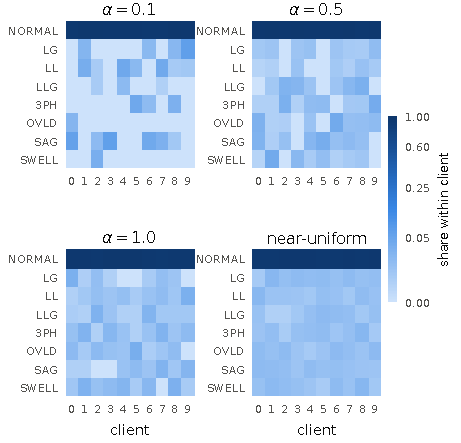
\includegraphics[width=\linewidth]{figures/fig_label_histogram}
\caption{Per-client share of each event class at $\alpha\in\{0.1,0.5,1.0\}$ and the near-uniform control, one panel per concentration, ten substations.}
\label{fig:labelhist}
\end{figure}

\begin{figure}[tbp]
\centering
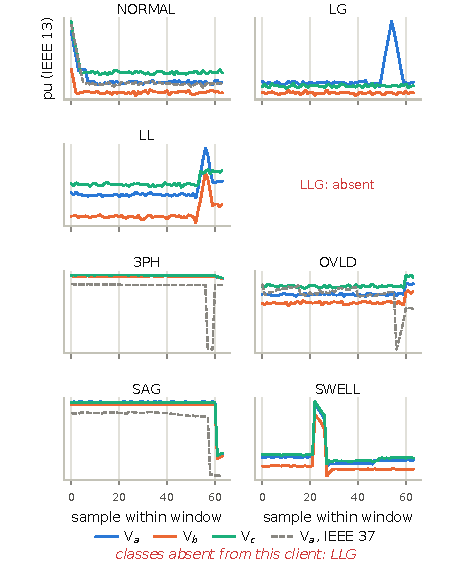
\includegraphics[width=\linewidth,height=0.85\textheight,keepaspectratio]{figures/fig_example_windows}
\caption{Representative $11\times64$ windows per event class: phase voltages after the measurement chain, with a cross-feeder reference trace in grey.}
\label{fig:windows}
\end{figure}

\section{Battery, provenance and pre-registration detail}
\label{sec:sup-design}

\subsection{The eighteen-arm reference frame and the attack grid}
\label{sec:sup-arms}

Federated results are only interpretable between two bounds, and the
surveyed application literature usually reports neither. Both are run:
a \emph{centralized ceiling} (pooled data -- the best a single model can
do if the privacy constraint were lifted) and a \emph{local-only floor}
(each substation training alone; mean, minimum and maximum over the ten
clients), beside plain FedAvg, FedProx, and the full pipeline with each
robust aggregator (Table~\ref{tab:arms}). A federated arm that beats the
floor buys something over isolation; the gap to the ceiling is the price
of decentralization, privacy and Byzantine tolerance.

\begin{table*}[tbp]
\centering
\caption{Reference-frame arms and attack-grid defense arms}
\label{tab:arms}
\scriptsize
\setlength{\tabcolsep}{2pt}%
\renewcommand{\arraystretch}{1.15}%
\begin{tabularx}{\linewidth}{@{}l l l L@{}}
\toprule
Arm & Mode & Aggregation & Role \\
\midrule
B1--B3 centralized      & pooled       & n.a. & accuracy ceiling \\
B4--B6 local-only       & per-client   & n.a. & accuracy floor \\
B7--B9 FedAvg           & federated    & weighted mean            & standard baseline \\
B10--B12 FedProx        & federated    & weighted mean ($\mu$ term) & heterogeneity baseline \\
B13--B15 pipeline-Krum  & federated    & fidelity+PBFT+Krum       & proposed \\
B16--B18 pipeline-geomed& federated    & fidelity+PBFT+geo-median & proposed \\
\midrule
no-defense             & federated    & weighted mean            & attack grid: what an undefended federation loses \\
Krum-alone             & federated    & Krum only                & attack grid: does agreement buy accuracy? \\
geomed-alone           & federated    & geo-median only          & attack grid: same question, averaging aggregator \\
fidelity-only          & federated    & gate + weighted mean     & ablation: the gate without agreement \\
\bottomrule
\end{tabularx}
\tablenota{Pipeline: fidelity $\rightarrow$ PBFT $\rightarrow$ robust aggregation (Algorithm~\ref{alg:pipeline}); \emph{alone}: the aggregator with no gate and no agreement layer. n.a.: no aggregation step.}
\end{table*}

One family is excluded, with a reason rather than silently:
root-dataset trust bootstrapping \cite{cao2021fltrust} assumes a clean
server-held dataset, which is unavailable by design in a multi-utility
federation.

\subsection{Battery composition and reconciliation}
\label{sec:sup-battery}

Table~\ref{tab:battery} enumerates the eleven battery blocks. Tier~1 --
the clean reference frame and the attack $\times$ defense grid --
carries the headline claims; Tier~2 carries the sensitivity sweeps and
ablations. Tier~3 is the \emph{control battery}, specified on 2026-07-31
after the pre-registered analysis was complete: two blocks that re-run
the entire Tier-1 grid under a contiguous chronological client split,
and one that sweeps the attacker's magnitude. It answers two threats to
validity the pre-registered design did not cover -- window overlap under
a random split, and the one attacker lever a scale-free gate cannot see.

\begin{table*}[tbp]
\centering
\caption{Battery composition after the X3 extension (merged, deduplicated corpus)}
\label{tab:battery}
\scriptsize
\setlength{\tabcolsep}{2pt}%
\renewcommand{\arraystretch}{1.15}%
\begin{tabularx}{\linewidth}{@{}l l L c@{}}
\toprule
Block & Tier & Grid & Runs \\
\midrule
T1a & 1 & 18-arm clean reference frame (6 arms $\times$ 3 models) & 270 \\
T1b & 1 & 4 attacks $\times$ 5 defense arms $\times$ 3 models, $f_{\mathrm{att}}=3/10$, $\alpha=0.5$ & 900 \\
T2a & 2 & $\alpha \in \{0.1, 1.0, \text{near-uniform}\}$ $\times$ \{FedAvg, pipeline-Krum\} $\times$ 3 models $\times$ \{clean, adaptive\} & 324 \\
T2b & 2 & $f_{\mathrm{att}} \in \{1,2\}/10$ $\times$ \{sign-flip, adaptive\} $\times$ \{no-defense, pipeline-Krum\} $\times$ 3 models & 216 \\
T2c & 2 & LDP $\sigma \in \{0.25,0.5,1,2\}$ $\times$ $\tau \in \{0.3,0.5,0.7\}$ $\times$ pipeline-Krum $\times$ 3 models & 324 \\
T2d & 2 & validators $M \in \{4,7\}$, $f=\lfloor(M-1)/3\rfloor$, $\times$ 3 models & 54 \\
T2e & 2 & ablations: SNN coding, SNN $T$ steps, FedProx $\mu$, fidelity-only, at 9 seeds & 189 \\
T3$\tau$ & 2 & fidelity threshold: 648 attack runs ($\tau\in\{0.6,0.8,1.0\}$ $\times$ 4 attacks $\times$ 3 models $\times$ 2 aggregators $\times$ 9 seeds) plus 324 local-DP runs (36 distinct $(\sigma,\tau,\text{model})$ cells $\times$ 9 seeds, emitted in exact triplicate and deduplicated semantically) & 972 \\
\midrule
\multicolumn{3}{@{}l}{\textbf{Pre-registered subtotal (extended)}} & \textbf{3{,}249} \\
\midrule
T1a\_temporal & 3 & post-registration control: block T1a re-run under the contiguous chronological split & 270 \\
T1b\_temporal & 3 & post-registration control: block T1b re-run under the same split & 900 \\
T4mag & 3 & post-registration control: attacker magnitude $s\in\{1,2,5,10\}$ $\times$ 4 defense arms $\times$ 3 models, adaptive-cosine at $f_{\mathrm{att}}=3/10$ & 432 \\
\midrule
\multicolumn{3}{@{}l}{\textbf{Control subtotal (leakage / magnitude, 2026-07-31)}} & \textbf{1{,}602} \\
\multicolumn{3}{@{}l}{\textbf{Total runs carrying a block label}} & \textbf{4{,}851} \\
\bottomrule
\end{tabularx}
\tablenota{\emph{Runs}: block inventory of \texttt{runs/summary.json}, matching the committed manifests except where noted in the text. Tier~1 and the temporal controls: 15 seeds; Tier~2 and Tier~3 controls: 9.}
\end{table*}

The five run batteries hold $6{,}836$ files between them: the $4{,}851$
distinct seeded runs above, plus six latency benchmarks behind
Table~\ref{tab:latency}; the gap between files and runs is re-execution,
and deduplication runs in two passes. First by \texttt{run\_id} -- the
X3 batteries re-ran the shared seeds ($0$--$4$ at Tier~1, $0$--$2$ at
Tier~2) under both fresh and inherited identifiers, and on a collision
the expansion copy wins ($5{,}535$ unique identifiers). Then on a
semantic configuration key, because the hash field in the expansion
manifests copies its seed line by convention: the T3$\tau$ manifest
re-emits each $(\sigma,\tau)$ cell once per source T2c threshold (exact
triplicates), and three Tier-2e state-space ablations (\texttt{ts4},
\texttt{ts16}, \texttt{codingrate}) are bit-identical configurations
measuring the same thing, so its $225$ files are $189$ distinct runs.
Six cells are recorded as \emph{diverged} and excluded from their cell
means: the pipeline+Krum state-space LDP runs at
$\sigma\in\{1.0,2.0\}$, $\tau\in\{0.8,1.0\}$, seeds 0 and 3
(Section~\ref{sec:res-ldp}). The control batteries are emitted by the
same manifest machinery -- each temporal run copies its T1 twin and
changes one field, so it pairs with its twin on every other axis.

The sweeps span six sensitivity families -- non-IID severity, attack
fraction, local-DP noise crossed with the admission threshold, validator
committee size, attack type, and arithmetic precision (an analytic
re-costing, with no training block of its own) -- and eight ablation
axes, of which the defense decomposition (none $\to$ fidelity-only $\to$
Krum-alone $\to$ pipeline-Krum $\to$ pipeline-geomed) carries the most
weight.

\subsection{Seeds, stated openly}
\label{sec:sup-seeds}

Tier~1 and the Tier-3 temporal controls run \textbf{15} seeds, and every
Tier-2 sweep and the Tier-3 magnitude control run \textbf{9}: the X3
coverage extension re-ran the shared seeds ($0$--$4$ at Tier~1,
$0$--$2$ at Tier~2) and added the new ones, taking the original $5$/$3$
plan -- itself reduced by a dated amendment before any Tier-1 run from
the 10 and 5 the project specified for itself, on a measured per-run
cost -- to fifteen and nine. The consequence, plainly: at fifteen paired
seeds an exact one-sided Wilcoxon signed-rank can reach $2^{-15}$, so
every pre-registered family is decidable at $\alpha=0.05$ after Holm
correction (the family floors are $7.3\times10^{-4}$ for H2,
$1.8\times10^{-4}$ for H3, $5.9\times10^{-3}$ for H5b), and the verdicts
are reads of the data rather than of the test's resolution. One seed
drives the \emph{entire} stochastic pipeline -- federation generation,
initialization, batching, DP noise, attack randomness and the PBFT
network draws -- so the repetitions are also independent dataset
re-draws, which is stronger than $k$-fold over a frozen split. The
extension also mixes two run environments: the original fleet (RTX
3060/3090/4080 class, torch 2.4--2.13) executed the pre-registered
seeds, while the X3 batteries ran on RTX 5090/4090 hardware under torch
2.9.1 -- the temporal cells therefore mix environments by construction,
and a subset analysis on the homogeneous seeds $5$--$14$ leaves the
headline conclusions unchanged.

\subsection{Attack settings}
\label{sec:sup-attacksettings}

Every attacker is constructed with \texttt{collude\_seed} equal to the
run seed, so all Byzantine clients draw the same $\omega$ per (seed,
round) -- one shared random direction, sign-fixed towards the damaging
half-space, that lands the coalition on a single point of the cone; the
per-attacker alternative ($\omega$ the component of $-h$ orthogonal to
$u$) is implemented but exercised by no run reported here. No manifest
entry overrides an attack default, so every attacked run uses target
score $\varsigma = 0.1$, safety margin $\eta = 0.15$, magnitude $s = 1$
(swept only in Section~\ref{sec:res-magnitude}), label-flip rate
$\mathrm{frac} = 1.0$ and $n_{\mathrm{peers}} = K = 10$, at Byzantine
fraction $f_{\mathrm{att}}/K = 0.3$ ($0.1$ and $0.2$ in block T2b).

\subsection{Pre-registration amendments}
\label{sec:sup-amendments}

Five hypotheses were registered before the first Tier-1 run, each with
its null, alternative, metric, test, correction family and decision rule
(summarized in the manuscript); two supporting claims are reported with
numbers rather than tests -- the latency envelope and the consensus
overhead (a lower bound) -- and a third, end-to-end ledger verification,
was registered but is \emph{not} instrumented in this battery's result
records, so it is reported as a design property with its test coverage
named, not as a measured result.

Deviations are recorded as dated amendments with reasons in the released
file; four are on record:
\begin{itemize}\setlength{\itemsep}{2pt}
\item \textbf{2026-07-30a}: an analysis-code fix restoring the
  state-space model to the H2, H3 and H5 test loops, changing no
  hypothesis, metric or test;
\item \textbf{2026-07-31a}: the statement that label-flip is realized as
  dynamic per-batch noise (manuscript threat-model section);
\item \textbf{2026-07-31b}: the Tier-3 control battery, added
  \emph{after} the registered analysis was complete -- it registers no
  hypothesis and changes no verdict, and its results are reported as
  post-hoc controls on the registered ones;
\item the \textbf{X3 coverage extension} that raised every cell's seed
  count -- it adds runs, not claims: no hypothesis, metric, test or
  decision rule moved.
\end{itemize}

\subsection{Provenance audit detail}
\label{sec:sup-provenance}

Every run serializes its complete configuration, its seed, its per-round
events, its final metrics, an environment fingerprint (framework and
CUDA versions, GPU name) and the git commit that produced it. That last
field is the honest weak point: it reads \texttt{unknown} in $5{,}366$
of the $5{,}535$ block-labelled records ($96.9\%$ -- $821$ of the $990$
records retained from the original battery, and every record of the
expansion), because most of the fleet ran from a working tree whose
commit was never captured. Per-run code provenance therefore rests on
the recorded configuration and environment fingerprint, on the
committed manifests and on seeded determinism, not on a commit id --
and the configuration hashes corroborate it where they can: $1{,}231$ of
the original battery's $1{,}845$ records ($66.7\%$) reproduce their
recorded hash under the canonical serializer and the other $614$ under
an auxiliary generator's non-canonical JSON encoding, same content,
different whitespace -- an inconsistency since fixed -- so on that
battery the audit found no configuration drift. The expansion's
manifests copy the seed line's hash by convention, so the canonical
audit does not cover them; their identity is the semantic configuration
key the corpus is deduplicated on. A same-seed CPU run is byte-identical
in its serialized result; bit-reproducibility is claimed \emph{on CPU
only}, because CUDA reductions are not deterministic -- the original
battery's $\tau$-sweep triplicates bound that residual: $24$ of its
$108$ groups differ across replicas at a median non-zero spread near
$10^{-4}$ \macroF{}, maximum $1.2\times10^{-3}$, while the extension's
are byte-identical. Property-based tests assert the invariants the
claims rest on -- aggregation permutation-invariance and exact
weighting, post-clip norm bounds, score range, ledger tamper detection,
and that the PBFT simulation commits exactly when $M \ge 3f+1$ and
otherwise fails closed -- alongside a golden fixed-seed regression
fixture. Training ran on a heterogeneous rented GPU fleet -- the
original battery on RTX 3060/3090/4080 hardware under torch 2.4--2.13,
the extension on RTX 5090/4090 under torch 2.9.1; \emph{all} latency
benchmarks ran on a single fixed reference machine while it was
otherwise idle. No model was quantized anywhere in this work: the INT8
rows are an analytic re-costing of the same operation counts with 8-bit
per-operation constants, and every measured latency is fp32.

\section{Additional results}
\label{sec:sup-results}

This section carries every display the manuscript's results section
references but could not hold, plus the complete statistical battery.
The organization follows the manuscript.

\subsection{The random-split reference frame and convergence}
\label{sec:sup-res-frame}

Table~\ref{tab:frame} is the pre-registered \emph{random-split}
reference frame -- the leakage-inflated diagnostic ceiling whose
leakage-controlled twin is the headline table of the manuscript.
Figure~\ref{fig:rounds} shows the round trajectories of the same
battery: only the CNN-LSTM FedAvg and FedProx arms reach $95\%$ of their
centralized ceiling inside the 30-round budget, and they do it on every
seed.

\begin{table*}[tbp]
\centering
\caption{Reference frame, random split (T1a, $\alpha=0.5$, no attack, 15 seeds)}
\label{tab:frame}
%% AUTO-GENERATED by `python -m experiments.report` -- do not hand-edit.
%% Schema: arm x model; macro-F1 mean, BCa CI, accuracy; rounds-to-target = first round reaching 95% of the same model's centralized ceiling
%% Every cell comes from a RunResult; a red numeric marker flags a value the
%% loaded runs cannot support, n.a. marks a structurally inapplicable cell.
%% Layout normalized to the group table template (tabular* full width, scriptsize, \tablenota).
\scriptsize
\setlength{\tabcolsep}{2pt}%
\renewcommand{\arraystretch}{1.15}%
\begin{tabular*}{\linewidth}{@{\extracolsep{\fill}}l l l c c c c@{}}
\toprule
 & Arm & Model & \macroF{} & BCa 95\% CI & Accuracy & Rounds to target \\
\midrule
B1--B3 & Centralized ceiling & CNN-LSTM & 0.582\,$\pm$\,0.100 & [0.535,\,0.633] & 0.555 & 1.7 \\
 &  & Spiking & 0.586\,$\pm$\,0.085 & [0.534,\,0.619] & 0.910 & 20.5 \\
 &  & Mamba & 0.849\,$\pm$\,0.049 & [0.823,\,0.871] & 0.973 & 9.6 \\
\midrule
B4--B6 & Local-only floor & CNN-LSTM & 0.292\,$\pm$\,0.028 & [0.031,\,0.493]$^{\dagger}$ & 0.760 & n.a. \\
 &  & Spiking & 0.129\,$\pm$\,0.008 & [0.049,\,0.212]$^{\dagger}$ & 0.597 & n.a. \\
 &  & Mamba & 0.197\,$\pm$\,0.013 & [0.106,\,0.359]$^{\dagger}$ & 0.760 & n.a. \\
\midrule
B7--B9 & FedAvg & CNN-LSTM & 0.600\,$\pm$\,0.048 & [0.578,\,0.625] & 0.955 & 16.3 \\
 &  & Spiking & 0.161\,$\pm$\,0.021 & [0.151,\,0.172] & 0.658 & n.r. \\
 &  & Mamba & 0.770\,$\pm$\,0.037 & [0.750,\,0.786] & 0.973 & 29.0$^{1/15}$ \\
\midrule
B10--B12 & FedProx ($\mu=0.01$) & CNN-LSTM & 0.603\,$\pm$\,0.056 & [0.579,\,0.635] & 0.955 & 17.0 \\
 &  & Spiking & 0.163\,$\pm$\,0.020 & [0.153,\,0.173] & 0.649 & n.r. \\
 &  & Mamba & 0.751\,$\pm$\,0.030 & [0.735,\,0.765] & 0.971 & 29.5$^{2/15}$ \\
\midrule
B13--B15 & Pipeline + Krum & CNN-LSTM & 0.476\,$\pm$\,0.069 & [0.441,\,0.510] & 0.896 & 20.8$^{4/15}$ \\
 &  & Spiking & 0.126\,$\pm$\,0.018 & [0.118,\,0.135] & 0.634 & n.r. \\
 &  & Mamba & 0.198\,$\pm$\,0.074 & [0.163,\,0.236] & 0.714 & n.r. \\
\midrule
B16--B18 & Pipeline + geomed & CNN-LSTM & 0.454\,$\pm$\,0.067 & [0.423,\,0.489] & 0.942 & 22.5$^{2/15}$ \\
 &  & Spiking & 0.136\,$\pm$\,0.019 & [0.127,\,0.145] & 0.651 & n.r. \\
 &  & Mamba & 0.156\,$\pm$\,0.048 & [0.135,\,0.181] & 0.738 & n.r. \\
\bottomrule
\end{tabular*}
\tablenota{Leakage-inflated diagnostic ceiling; the headline frame is Table~\ref{tab:temporal_frame}. Pooled test set, mean over seeds, BCa 95\% CI. $^{\dagger}$Local-only: per-client $[\min,\max]$ over the ten substations, not a CI. Centralized ceilings use the federated arms' loss and threshold (recipe-matched).}
\end{table*}

\begin{figure}[tbp]
\centering
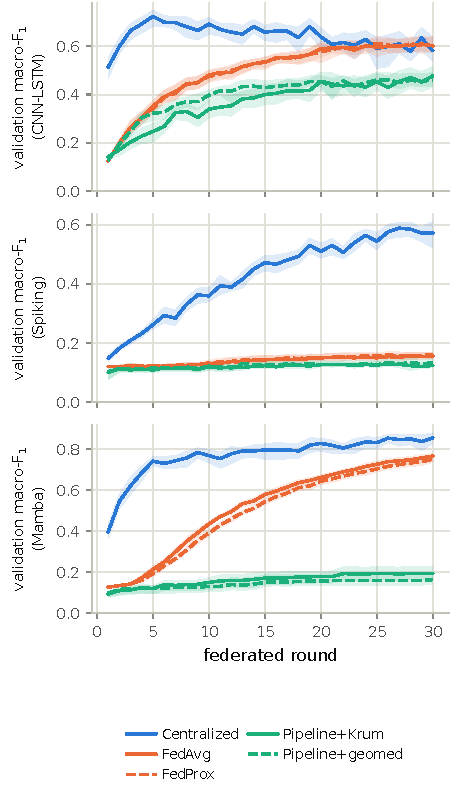
\includegraphics[width=\linewidth,height=0.85\textheight,keepaspectratio]{figures/fig_rounds}
\caption{Validation \macroF{} per federated round (BCa bands), one panel per model (T1a, random split, 15 seeds); trivial-predictor floor \macroF{}~$0.121$.}
\label{fig:rounds}
\end{figure}

\subsection{The shallow probe and the frequency-deviation audit}
\label{sec:sup-probe}

A deep model is only justified if a cheap one cannot do the job, so a
shallow gradient-boosted tree was scored on the same five federations --
\textsc{HistGradientBoosting} at library defaults, no tuning, over $77$
summary-statistic features per window (seven per channel), in fits of
$1$--$4$\,s. Pooled, it reaches \macroF{} $0.692 \pm 0.042$ on the same
global test set and $0.318$ trained per substation; under the
chronological cut it falls $23\%$ to $0.533 \pm 0.063$ -- level with the
CNN-LSTM centralized ceiling under either protocol and far below Mamba,
though the CNN-LSTM's \emph{federated} arm ($0.596$) still edges the
pooled probe under the same split. One disclosure weakens that headline:
the $0.692$ depends on \textsc{scikit-learn}'s default early stopping,
which halts the fit at $11$ of $100$ boosting iterations -- disabled,
the same probe scores $0.275 \pm 0.095$. The reading survives both
protocols: the reference architecture is not justified by its
\emph{centralized} accuracy -- its case is timing -- and the benchmark
demands deep learning only at the level the state-space model reaches.

The same probe audits the sharpest shortcut the benchmark offers. The
synthetic $f_{\mathrm{dev}}$ channel is coupled to event class by
construction and could act as a label fingerprint; dropping it costs
$-0.011$ \macroF{} under the random split and $-0.027$ under the
chronological one, both intervals spanning zero, while the channel alone
reaches $0.295$ and $0.234$ -- real but far-from-sufficient signal
(Table~\ref{tab:fdev}; three limits bound the reading: a shallow probe,
not the deep models, whose capacity to exploit a subtle coupling is
larger; a test with no power at $n=5$; and an argument that therefore
rests on the magnitude of the change, not its $p$-value).

\begin{table}[tbp]
\centering
\caption{Frequency-deviation ablation on the shallow probe (5 federations)}
\label{tab:fdev}
\scriptsize
\setlength{\tabcolsep}{2pt}%
\renewcommand{\arraystretch}{1.15}%
\begin{tabular*}{\linewidth}{@{\extracolsep{\fill}}l c c c c@{}}
\toprule
Split & $\Delta$\macroF{} & BCa 95\% CI & $p$ & $f_{\mathrm{dev}}$ only \\
\midrule
Random & $-0.011$ & $[-0.061,\,+0.044]$ & $0.81$ & $0.295$ \\
Temporal & $-0.027$ & $[-0.101,\,+0.053]$ & $0.625$ & $0.234$ \\
\bottomrule
\end{tabular*}
\tablenota{$\Delta$\macroF{}: paired change from dropping the seven $f_{\mathrm{dev}}$ features; \emph{$f_{\mathrm{dev}}$ only}: refit on those seven alone (majority floor $0.121$; all channels $0.692$ random, $0.533$ temporal). At $n=5$ the exact two-sided Wilcoxon $p$ cannot fall below $0.0625$.}
\end{table}

\subsection{The random-split attack grid}
\label{sec:sup-res-attack}

Table~\ref{tab:attackdefense} is the attack $\times$ defense grid under
the pre-registered random split, at the tolerance-limit attack fraction;
its chronological-split counterpart is the headline attack table of the
manuscript, printed with the cell-by-cell change against this one.
Figure~\ref{fig:cd} summarizes the multi-arm ranking behind the
manuscript's H2 discussion: geometric-median aggregation standing alone
attains the best average rank, both full-pipeline arms rank below it, and
no-defense is not separated from pipeline+Krum, so the admission pipeline
does not improve on robust averaging. The per-seed blocking ($n=180$)
separates eight of the ten pairs and preserves this ordering.

\begin{table*}[tbp]
\centering
\caption{Attack $\times$ defense \macroF{} (mean $\pm$ sd), random split (T1b, $f_{\mathrm{att}}=3/10$, $\alpha=0.5$, 15 seeds)}
\label{tab:attackdefense}
%% AUTO-GENERATED by `python -m experiments.report` -- do not hand-edit.
%% Schema: defense arm x model rows; one column per attack (macro-F1 mean +/- sd over seeds)
%% Every cell comes from a RunResult; a red numeric marker flags a value the
%% loaded runs cannot support, n.a. marks a structurally inapplicable cell.
%% Layout normalized to the group table template (tabular* full width, scriptsize, \tablenota).
\scriptsize
\setlength{\tabcolsep}{2pt}%
\renewcommand{\arraystretch}{1.15}%
\begin{tabular*}{\linewidth}{@{\extracolsep{\fill}}l l c c c c c@{}}
\toprule
Defense arm & Model & Clean & Sign-flip & Gaussian & Label-flip$^{\dagger}$ & Adaptive \\
\midrule
No defense & CNN-LSTM & 0.600\,$\pm$\,0.048 & 0.392\,$\pm$\,0.063 & 0.059\,$\pm$\,0.017 & 0.509\,$\pm$\,0.069 & 0.629\,$\pm$\,0.057 \\
 & Spiking & 0.161\,$\pm$\,0.021 & 0.124\,$\pm$\,0.012 & 0.100\,$\pm$\,0.029 & 0.093\,$\pm$\,0.028 & 0.152\,$\pm$\,0.018 \\
 & Mamba & 0.770\,$\pm$\,0.037 & 0.293\,$\pm$\,0.059 & 0.076\,$\pm$\,0.010 & 0.418\,$\pm$\,0.036 & 0.739\,$\pm$\,0.054 \\
\midrule
Krum alone & CNN-LSTM & n.a. & 0.355\,$\pm$\,0.095 & 0.408\,$\pm$\,0.101 & 0.359\,$\pm$\,0.074 & 0.100\,$\pm$\,0.050 \\
 & Spiking & n.a. & 0.128\,$\pm$\,0.020 & 0.137\,$\pm$\,0.024 & 0.124\,$\pm$\,0.024 & 0.060\,$\pm$\,0.062 \\
 & Mamba & n.a. & 0.224\,$\pm$\,0.060 & 0.261\,$\pm$\,0.042 & 0.245\,$\pm$\,0.052 & 0.043\,$\pm$\,0.033 \\
\midrule
Geo-median alone & CNN-LSTM & n.a. & 0.437\,$\pm$\,0.060 & 0.587\,$\pm$\,0.043 & 0.544\,$\pm$\,0.069 & 0.609\,$\pm$\,0.070 \\
 & Spiking & n.a. & 0.132\,$\pm$\,0.013 & 0.151\,$\pm$\,0.017 & 0.103\,$\pm$\,0.025 & 0.149\,$\pm$\,0.018 \\
 & Mamba & n.a. & 0.389\,$\pm$\,0.071 & 0.692\,$\pm$\,0.060 & 0.439\,$\pm$\,0.039 & 0.726\,$\pm$\,0.037 \\
\midrule
Pipeline + Krum & CNN-LSTM & 0.476\,$\pm$\,0.069 & 0.323\,$\pm$\,0.069 & 0.366\,$\pm$\,0.076 & 0.368\,$\pm$\,0.065 & 0.235\,$\pm$\,0.088 \\
 & Spiking & 0.126\,$\pm$\,0.018 & 0.097\,$\pm$\,0.039 & 0.106\,$\pm$\,0.029 & 0.095\,$\pm$\,0.042 & 0.095\,$\pm$\,0.036 \\
 & Mamba & 0.198\,$\pm$\,0.074 & 0.076\,$\pm$\,0.048 & 0.089\,$\pm$\,0.057 & 0.110\,$\pm$\,0.056 & 0.031\,$\pm$\,0.025 \\
\midrule
Pipeline + geomed & CNN-LSTM & 0.454\,$\pm$\,0.067 & 0.320\,$\pm$\,0.051 & 0.377\,$\pm$\,0.056 & 0.357\,$\pm$\,0.132 & 0.420\,$\pm$\,0.140 \\
 & Spiking & 0.136\,$\pm$\,0.019 & 0.097\,$\pm$\,0.039 & 0.106\,$\pm$\,0.028 & 0.091\,$\pm$\,0.031 & 0.082\,$\pm$\,0.048 \\
 & Mamba & 0.156\,$\pm$\,0.048 & 0.076\,$\pm$\,0.048 & 0.084\,$\pm$\,0.050 & 0.095\,$\pm$\,0.049 & 0.051\,$\pm$\,0.030 \\
\bottomrule
\end{tabular*}
\tablenota{$^{\dagger}$Realized as dynamic per-batch label noise; see Section~\ref{sec:threat}.}

\end{table*}

\begin{figure}[tbp]
\centering
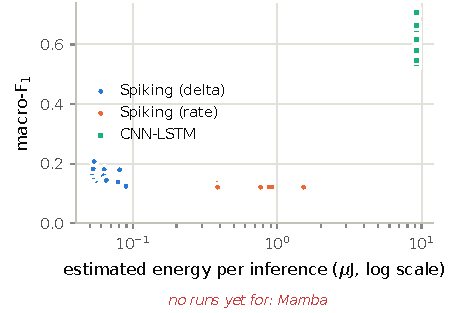
\includegraphics[width=\linewidth]{figures/fig_energy_accuracy}
\caption{Estimated energy per inference (log scale) against \macroF{} (BCa intervals) for both spiking codings, CNN-LSTM and Mamba. Energy is an arithmetic-only estimate.}
\label{fig:energyacc}
\end{figure}

\begin{figure*}[tbp]
\centering
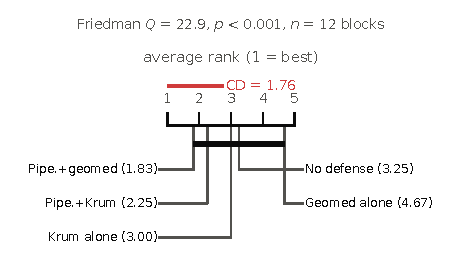
\includegraphics[width=0.88\linewidth]{figures/fig_cd_diagram}
\caption{Nemenyi critical-difference diagram over the five defense arms, pre-registered blocking by (attack $\times$ model) seed means ($n=12$, CD $=1.76$); bars join indistinguishable arms.}
\label{fig:cd}
\end{figure*}

\subsection{Defense decomposition}
\label{sec:sup-res-decomp}

Table~\ref{tab:decomp} decomposes the defense one rung at a time under
the defense-aware attacker. Geometric-median aggregation \emph{alone}
preserves accuracy almost perfectly while rejecting no honest client,
whereas the same aggregator behind the gate and PBFT drops sharply and
rejects most honest updates; Krum alone is worse than useless -- the
single-update selector is exactly what the cosine-aligned attacker
games.

\begin{table*}[tbp]
\centering
\caption{Defense decomposition, rung by rung, under the defense-aware attacker (random split)}
\label{tab:decomp}
%% AUTO-GENERATED by `python -m experiments.report` -- do not hand-edit.
%% Schema: defense rung x model under the adaptive attacker; admission/FRR are measured at the fidelity+PBFT gate and read `--' on the rungs that have no gate, where 1.000/0.000 would be a definition rather than a measurement; the ledger column is `--' throughout because Ledger.verify() is not instrumented in the RunResults
%% Every cell comes from a RunResult; a red numeric marker flags a value the
%% loaded runs cannot support, n.a. marks a structurally inapplicable cell.
%% Layout normalized to the group table template (tabular* full width, scriptsize, \tablenota).
\scriptsize
\setlength{\tabcolsep}{2pt}%
\renewcommand{\arraystretch}{1.15}%
\begin{tabular*}{\linewidth}{@{\extracolsep{\fill}}l l c c c c c@{}}
\toprule
Defense rung & Model & \macroF{} & $\Delta$ vs none & Attacker adm. & Honest FRR & Ledger \\
\midrule
No defense & CNN-LSTM & 0.629\,$\pm$\,0.057 & n.a. & n.a. & n.a. & n.a. \\
 & Spiking & 0.152\,$\pm$\,0.018 & n.a. & n.a. & n.a. & n.a. \\
 & Mamba & 0.739\,$\pm$\,0.054 & n.a. & n.a. & n.a. & n.a. \\
\midrule
Fidelity gate only & CNN-LSTM & 0.396\,$\pm$\,0.110 & $-$0.233 & 0.606 & 0.711 & n.a. \\
 & Spiking & 0.106\,$\pm$\,0.034 & $-$0.047 & 0.759 & 0.744 & n.a. \\
 & Mamba & 0.064\,$\pm$\,0.038 & $-$0.675 & 0.856 & 0.964 & n.a. \\
\midrule
Krum alone & CNN-LSTM & 0.100\,$\pm$\,0.050 & $-$0.529 & n.a. & n.a. & n.a. \\
 & Spiking & 0.060\,$\pm$\,0.062 & $-$0.093 & n.a. & n.a. & n.a. \\
 & Mamba & 0.043\,$\pm$\,0.033 & $-$0.696 & n.a. & n.a. & n.a. \\
\midrule
Geo-median alone & CNN-LSTM & 0.609\,$\pm$\,0.070 & $-$0.020 & n.a. & n.a. & n.a. \\
 & Spiking & 0.149\,$\pm$\,0.018 & $-$0.003 & n.a. & n.a. & n.a. \\
 & Mamba & 0.726\,$\pm$\,0.037 & $-$0.013 & n.a. & n.a. & n.a. \\
\midrule
Fidelity + PBFT + Krum & CNN-LSTM & 0.235\,$\pm$\,0.088 & $-$0.394 & 0.549 & 0.691 & n.a. \\
 & Spiking & 0.095\,$\pm$\,0.036 & $-$0.057 & 0.557 & 0.705 & n.a. \\
 & Mamba & 0.031\,$\pm$\,0.025 & $-$0.709 & 0.846 & 0.972 & n.a. \\
\midrule
Fidelity + PBFT + geomed & CNN-LSTM & 0.420\,$\pm$\,0.140 & $-$0.209 & 0.534 & 0.657 & n.a. \\
 & Spiking & 0.082\,$\pm$\,0.048 & $-$0.070 & 0.578 & 0.660 & n.a. \\
 & Mamba & 0.051\,$\pm$\,0.030 & $-$0.688 & 0.846 & 0.969 & n.a. \\
\bottomrule
\end{tabular*}
\tablenota{Admission and honest FRR exist only on gated rungs (fidelity-only and both pipelines); n.a. elsewhere, where they hold by definition. Ledger: n.a. throughout, since no run verifies the hash chain end to end (property tests only).}
\end{table*}

\subsection{Defense-aware evasion, in full}
\label{sec:sup-res-adaptive}

\begin{table*}[tbp]
\centering
\caption{Evasion and damage per attack and aggregator (T1b, random split, 15 seeds)}
\label{tab:adaptive}
%% AUTO-GENERATED by `python -m experiments.report` -- do not hand-edit.
%% Schema: aggregator x attack x model; realised attacker fidelity score vs tau, gate admission, honest FRR and the paired macro-F1 drop
%% Every cell comes from a RunResult; a red numeric marker flags a value the
%% loaded runs cannot support, n.a. marks a structurally inapplicable cell.
%% Layout normalized to the group table template (tabular* full width, scriptsize, \tablenota).
\scriptsize
\setlength{\tabcolsep}{2pt}%
\renewcommand{\arraystretch}{1.15}%
\begin{tabular*}{\linewidth}{@{\extracolsep{\fill}}l l l c c c c@{}}
\toprule
Aggregator & Attack & Model & Mean score & Admission & Honest FRR & $\Delta$\macroF{} \\
\midrule
Krum & Sign-flip & CNN-LSTM & 1.046 & 0.000 & 0.890 & 0.153 \\
 &  & Spiking & 1.026 & 0.000 & 0.958 & 0.028 \\
 &  & Mamba & 0.978 & 0.000 & 0.997 & 0.122 \\
 & Adaptive cosine & CNN-LSTM & 0.503 & 0.545 & 0.708 & 0.242 \\
 &  & Spiking & 0.489 & 0.568 & 0.702 & 0.030 \\
 &  & Mamba & 0.407 & 0.870 & 0.975 & 0.167 \\
\midrule
Geo-median & Sign-flip & CNN-LSTM & 1.019 & 0.000 & 0.920 & 0.134 \\
 &  & Spiking & 1.015 & 0.000 & 0.971 & 0.039 \\
 &  & Mamba & 0.975 & 0.000 & 0.997 & 0.079 \\
 & Adaptive cosine & CNN-LSTM & 0.552 & 0.530 & 0.673 & 0.034 \\
 &  & Spiking & 0.532 & 0.589 & 0.655 & 0.054 \\
 &  & Mamba & 0.397 & 0.870 & 0.972 & 0.105 \\
\bottomrule
\end{tabular*}

\tablenota{Score: realized fidelity of attacker updates, mean over rounds and seeds; round~1 excluded, since the adaptive attacker then submits its honest direction (Section~\ref{sec:threat}).}
\end{table*}

\subsection{The admission-threshold sweep}
\label{sec:sup-res-tau}

The pre-registered threshold is one point on a curve, and sweeping it
changes the diagnosis (Table~\ref{tab:tau_sweep}). As $\tau$ opens from
$0.5$ to $1.0$ the gate stops rejecting honest clients -- false-rejection
falls from $0.68$--$0.97$ at $\tau=0.5$ to $0.11$ or less at $\tau=0.8$
and to $0.016$ or less at $\tau=1.0$ -- while the defense-aware attacker
is admitted essentially always (admission $\ge 0.92$ everywhere at
$\tau \ge 0.8$). Behind the geometric median accuracy \emph{recovers} as
the gate opens: averaged over the three models, \macroF{} rises from
$0.184$ at $\tau=0.5$ to $0.487$ at $\tau=1.0$, and Mamba -- the arm the
gate damages most, at $0.051$ under the pre-registered calibration --
climbs to $0.718$, within $0.01$ of geo-median-alone
(Table~\ref{tab:decomp}). Behind Krum it collapses further, $0.120
\rightarrow 0.069$: with a wide-open gate, Krum is again selecting a
single update out of a cloud the cosine-aligned attacker was shaped to
sit inside. At $\tau=0.5$ the gate was throttling its own aggregator,
discarding most of the honest updates a robust average needs in order to
be robust; released, and paired with an averaging-style aggregator, it
costs little -- $\tau \approx 1.0$ with geometric median is
approximately geo-median-alone, with the admission decision still
jointly witnessed and written to the chain. The negative result is about
calibration rather than mechanism: at the pre-registered operating point
the pipeline subtracts accuracy, and no setting of $\tau$ makes it
\emph{add} any over the bare aggregator.

\begin{table*}[tbp]
\centering
\caption{Admission-threshold sweep under the defense-aware attacker (random split)}
\label{tab:tau_sweep}
%% AUTO-GENERATED by `python -m experiments.report` -- do not hand-edit.
%% Schema: admission threshold tau x model under the adaptive-cosine attacker (30% Byzantine, no LDP noise); tau=0.5 is the reference frame (block T1b, 15 seeds), tau in {0.6,0.8,1.0} is block T3tau (9 seeds); the fidelity gate is identical in both pipeline arms so FRR / admission / score pool over them, while macro-F1 is split by aggregator because that is where the arms differ; round 1 is excluded from the attacker's score (it has no aggregate to aim at)
%% Every cell comes from a RunResult; a red numeric marker flags a value the
%% loaded runs cannot support, n.a. marks a structurally inapplicable cell.
%% Layout normalized to the group table template (tabular* full width, scriptsize, \tablenota).
\scriptsize
\setlength{\tabcolsep}{2pt}%
\renewcommand{\arraystretch}{1.15}%
\begin{tabular*}{\linewidth}{@{\extracolsep{\fill}}l l c c c c c@{}}
\toprule
$\tau$ & Model & Honest FRR & Attacker adm. & Attacker score & \macroF{} Krum & \macroF{} geo-med \\
\midrule
0.5 & CNN-LSTM & 0.691 & 0.537 & 0.528 & 0.235 & 0.420 \\
 & Spiking & 0.678 & 0.579 & 0.511 & 0.095 & 0.082 \\
 & Mamba & 0.974 & 0.870 & 0.402 & 0.031 & 0.051 \\
\midrule
0.6 & CNN-LSTM & 0.425 & 0.701 & 0.491 & 0.171 & 0.274 \\
 & Spiking & 0.438 & 0.686 & 0.539 & 0.091 & 0.072 \\
 & Mamba & 0.852 & 1.000 & 0.368 & 0.054 & 0.031 \\
\midrule
0.8 & CNN-LSTM & 0.082 & 0.925 & 0.394 & 0.109 & 0.584 \\
 & Spiking & 0.111 & 0.937 & 0.310 & 0.055 & 0.141 \\
 & Mamba & 0.064 & 1.000 & 0.299 & 0.056 & 0.643 \\
\midrule
1.0 & CNN-LSTM & 0.000 & 0.987 & 0.374 & 0.061 & 0.599 \\
 & Spiking & 0.016 & 0.969 & 0.306 & 0.091 & 0.145 \\
 & Mamba & 0.000 & 1.000 & 0.287 & 0.056 & 0.718 \\
\bottomrule
\end{tabular*}
\tablenota{Gate columns pool both pipelines, which share the admission stage. $\tau=0.5$: T1b (15 seeds); $\tau\in\{0.6,0.8,1.0\}$: T3$\tau$ (9 seeds). No local DP here (the $\sigma\times\tau$ grid is Table~\ref{tab:ldp}); no diverged runs.}
\end{table*}

\subsection{Heterogeneity sweep}
\label{sec:sup-res-alpha}

\begin{table*}[tbp]
\centering
\caption{Non-IID severity sweep (T2a, random split, 9 seeds)}
\label{tab:alpha}
%% AUTO-GENERATED by `python -m experiments.report` -- do not hand-edit.
%% Schema: alpha x arm; clean and adaptive-attack columns per model
%% Every cell comes from a RunResult; a red numeric marker flags a value the
%% loaded runs cannot support, n.a. marks a structurally inapplicable cell.
%% Layout normalized to the group table template (tabular* full width, scriptsize, \tablenota).
\scriptsize
\setlength{\tabcolsep}{2pt}%
\renewcommand{\arraystretch}{1.15}%
\begin{tabular*}{\linewidth}{@{\extracolsep{\fill}}l l c c c c c c@{}}
\toprule
 & & \multicolumn{2}{c}{CNN-LSTM} & \multicolumn{2}{c}{Spiking} & \multicolumn{2}{c}{Mamba} \\
\cmidrule(lr){3-4}\cmidrule(lr){5-6}\cmidrule(lr){7-8}
$\alpha$ & Arm & Clean & Adaptive & Clean & Adaptive & Clean & Adaptive \\
\midrule
0.1 & FedAvg & 0.499 & 0.532 & 0.118 & 0.123 & 0.798 & 0.687 \\
 & Pipeline + Krum & 0.300 & 0.171 & 0.113 & 0.091 & 0.206 & 0.051 \\
\midrule
0.5$^{\ast}$ & FedAvg & 0.600 & 0.629 & 0.161 & 0.152 & 0.770 & 0.739 \\
 & Pipeline + Krum & 0.476 & 0.235 & 0.126 & 0.095 & 0.198 & 0.031 \\
\midrule
1.0 & FedAvg & 0.649 & 0.630 & 0.170 & 0.171 & 0.757 & 0.744 \\
 & Pipeline + Krum & 0.477 & 0.233 & 0.131 & 0.100 & 0.180 & 0.030 \\
\midrule
near-uniform & FedAvg & 0.683 & 0.629 & 0.190 & 0.199 & 0.770 & 0.763 \\
 & Pipeline + Krum & 0.556 & 0.282 & 0.139 & 0.109 & 0.279 & 0.050 \\
\bottomrule
\end{tabular*}
\tablenota{$^{\ast}$Reference-frame value (block T1a).}

\tablenota{Near-uniform: a near-uniform Dirichlet draw, not an exact uniform sampler.}
\end{table*}

\subsection{Consensus overhead}
\label{sec:sup-res-consensus}

\begin{table*}[tbp]
\centering
\caption{Consensus cost against committee size $M$ (random split)}
\label{tab:consensus}
%% AUTO-GENERATED by `python -m experiments.report` -- do not hand-edit.
%% Schema: committee-size sweep on the pipeline+Krum arm UNDER THE ADAPTIVE-COSINE ATTACKER (30% Byzantine) -- the macro-F1 columns are attacked accuracies, not clean ones; message count observed per committing round, latency simulated from the utility-WAN lognormal (a lower bound); M=10 is read from block T1b, M in {4,7} from T2d
%% Every cell comes from a RunResult; a red numeric marker flags a value the
%% loaded runs cannot support, n.a. marks a structurally inapplicable cell.
%% Layout normalized to the group table template (tabular* full width, scriptsize, \tablenota).
\scriptsize
\setlength{\tabcolsep}{2pt}%
\renewcommand{\arraystretch}{1.15}%
\begin{tabular*}{\linewidth}{@{\extracolsep{\fill}}l c c c c c c c@{}}
\toprule
 & & & \multicolumn{2}{c}{Sim.\ latency (ms)} & \multicolumn{3}{c}{\macroF{} under attack$^{\dagger}$} \\
\cmidrule(lr){4-5}\cmidrule(lr){6-8}
$M$ & $f$ & Messages/round & p50 & p95 & CNN-LSTM & Spiking & Mamba \\
\midrule
4 & 1 & 24 & 113.4 & 158.6 & 0.210 & 0.103 & 0.023 \\
7 & 2 & 84 & 145.4 & 199.5 & 0.220 & 0.106 & 0.024 \\
10 & 3 & 180 & 167.8 & 221.2 & 0.235 & 0.095 & 0.031 \\
\bottomrule
\end{tabular*}
\tablenota{$^{\dagger}$Under the adaptive attacker (30\% Byzantine) on pipeline+Krum; not comparable with the clean frame. $M=10$: T1b (15 seeds); $M\in\{4,7\}$: T2d (9 seeds). Messages and latency do not depend on the attack. \textbf{Lower bound}: always-honest primary, no view change; batching, checkpointing and authentication not modelled.}
\end{table*}

\subsection{The full local-DP operating grid}
\label{sec:sup-res-ldp}

Table~\ref{tab:ldp} is the pre-registered twelve-point $(\sigma,\tau)$
local-DP grid; its extension to $\tau=1.0$ is the frontier table of the
manuscript.

\begin{table*}[tbp]
\centering
\caption{Local-DP operating grid, $\sigma\times\tau$ (T2c, random split, 9 seeds)}
\label{tab:ldp}
%% AUTO-GENERATED by `python -m experiments.report` -- do not hand-edit.
%% Schema: tau x sigma grid; epsilon is computed by RDP composition, not measured
%% Every cell comes from a RunResult; a red numeric marker flags a value the
%% loaded runs cannot support, n.a. marks a structurally inapplicable cell.
%% Layout normalized to the group table template (tabular* full width, scriptsize, \tablenota).
\scriptsize
\setlength{\tabcolsep}{2pt}%
\renewcommand{\arraystretch}{1.15}%
\begin{tabular*}{\linewidth}{@{\extracolsep{\fill}}l c c c c c c c@{}}
\toprule
 & & & & & \multicolumn{3}{c}{\macroF{}} \\
\cmidrule(lr){6-8}
$\tau$ & $\sigma$ & $\varepsilon$ & Honest FRR & Attacker adm. & CNN-LSTM & Spiking & Mamba \\
\midrule
0.3 & 0.25 & 345 & 1.000 & 0.000 & 0.024 & 0.040 & 0.033 \\
0.3 & 0.5 & 113 & 1.000 & 0.000 & 0.024 & 0.040 & 0.033 \\
0.3 & 1.0 & 41.3 & 1.000 & 0.000 & 0.024 & 0.040 & 0.033 \\
0.3 & 2.0 & 16.9 & 1.000 & 0.000 & 0.024 & 0.040 & 0.033 \\
\midrule
0.5 & 0.25 & 345 & 1.000 & 0.000 & 0.024 & 0.040 & 0.033 \\
0.5 & 0.5 & 113 & 1.000 & 0.000 & 0.024 & 0.040 & 0.033 \\
0.5 & 1.0 & 41.3 & 1.000 & 0.000 & 0.024 & 0.040 & 0.033 \\
0.5 & 2.0 & 16.9 & 1.000 & 0.000 & 0.024 & 0.040 & 0.033 \\
\midrule
0.7 & 0.25 & 345 & 1.000 & 0.000 & 0.024 & 0.040 & 0.033 \\
0.7 & 0.5 & 113 & 1.000 & 0.000 & 0.024 & 0.040 & 0.033 \\
0.7 & 1.0 & 41.3 & 1.000 & 0.000 & 0.024 & 0.040 & 0.033 \\
0.7 & 2.0 & 16.9 & 1.000 & 0.000 & 0.024 & 0.040 & 0.033 \\
\bottomrule
\end{tabular*}

\tablenota{$\varepsilon$: R\'enyi composition over 30 rounds at $\delta=10^{-5}$ (Eq.~\ref{eq:epsilon}); a computed guarantee, not a measurement.}
\end{table*}

\subsection{Latency distributions}
\label{sec:sup-res-latency}

\begin{figure*}[tbp]
\centering
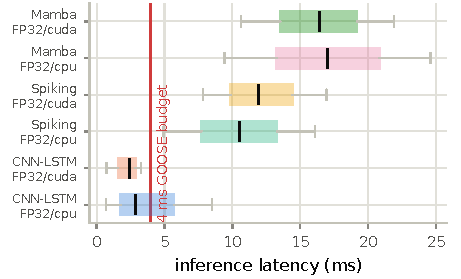
\includegraphics[width=\linewidth]{figures/fig_latency_goose}
\caption{Measured inference-latency distributions per model, precision and device, with p50/p95/p99 marked; vertical line: 4\,ms fast-message envelope.}
\label{fig:latency}
\end{figure*}

\subsection{Ablations, in full}
\label{sec:sup-res-ablations}

Tables~\ref{tab:coding} and~\ref{tab:fedprox} carry the ablation
grids. Under delta coding, shortening the unroll helps -- $T=4$ gives
the best clean \macroF{} at $0.204$, ahead of $T=8$ ($0.161$) and $T=16$
($0.132$), and at nine seeds the ordering is pairwise significant -- so
longer temporal integration buys more SynOps and energy for \emph{less}
accuracy, and rate coding pins at the $0.121$ trivial floor regardless
of unroll. FedProx is inert: judged against the \emph{paired} FedAvg
baseline (the $\mu \in \{0.001, 0.1\}$ rows run nine seeds against the
fifteen-seed reference), no proximal weight moves any model beyond seed
noise (largest paired gain $+0.006$), and the largest weight resolves
the harm it always suggested (Mamba at $\mu = 0.1$: $0.614$ against a
paired $0.764$).

\begin{table*}[tbp]
\centering
\caption{Spiking input-coding and unroll-length ablation (T2e, random split, 9 seeds)}
\label{tab:coding}
%% AUTO-GENERATED by `python -m experiments.report` -- do not hand-edit.
%% Schema: spiking coding x unroll length T; clean and adaptive macro-F1 + energy
%% Every cell comes from a RunResult; a red numeric marker flags a value the
%% loaded runs cannot support, n.a. marks a structurally inapplicable cell.
%% Layout normalized to the group table template (tabular* full width, scriptsize, \tablenota).
\scriptsize
\setlength{\tabcolsep}{2pt}%
\renewcommand{\arraystretch}{1.15}%
\begin{tabular*}{\linewidth}{@{\extracolsep{\fill}}l c c c c c@{}}
\toprule
Coding & $T$ & \macroF{} clean & \macroF{} adaptive & SynOps/inf. & Est.\ \uJ{}/inf. \\
\midrule
rate & 4 & 0.122 & 0.121 & 422\,827 & 0.381 \\
rate & 8 & 0.121 & 0.121 & 849\,521 & 0.765 \\
rate & 16 & 0.121 & 0.121 & 1\,693\,432 & 1.52 \\
\midrule
delta & 4 & 0.204 & 0.192 & 47\,681 & 0.0429 \\
delta & 8 & 0.161 & 0.152 & 70\,079 & 0.0631 \\
delta & 16 & 0.132 & 0.121 & 133\,153 & 0.120 \\
\bottomrule
\end{tabular*}

\tablenota{Energy is the arithmetic-only SynOps estimate per inference.}
\end{table*}

\begin{table*}[tbp]
\centering
\caption{FedProx proximal-weight ablation against paired FedAvg (random split)}
\label{tab:fedprox}
%% AUTO-GENERATED by `python -m experiments.report` -- do not hand-edit.
%% Schema: FedProx proximal-weight sweep against FedAvg, three models; the block each row comes from is in its mu label (T1a = 15 seeds, T2e = 9 seeds) and the Delta column is a paired difference over the seeds the row and FedAvg share, so it subtracts the *paired* FedAvg column beside it, never the 15-seed absolute mean
%% Every cell comes from a RunResult; a red numeric marker flags a value the
%% loaded runs cannot support, n.a. marks a structurally inapplicable cell.
%% Layout normalized to the group table template (tabular* full width, scriptsize, \tablenota).
\scriptsize
\setlength{\tabcolsep}{2pt}%
\renewcommand{\arraystretch}{1.15}%
\begin{tabular*}{\linewidth}{@{\extracolsep{\fill}}l l c c c c@{}}
\toprule
$\mu$ & Model & \macroF{} & BCa 95\% CI & FedAvg (paired) & $\Delta$ vs FedAvg \\
\midrule
FedAvg ($\mu=0$) & CNN-LSTM & 0.600\,$\pm$\,0.048 & [0.578,\,0.625] & n.a. & n.a. \\
 & Spiking & 0.161\,$\pm$\,0.021 & [0.151,\,0.172] & n.a. & n.a. \\
 & Mamba & 0.770\,$\pm$\,0.037 & [0.750,\,0.786] & n.a. & n.a. \\
\midrule
0.001 & CNN-LSTM & 0.596\,$\pm$\,0.064 & [0.563,\,0.644] & 0.5922$^{9}$ & $+$0.004 \\
 & Spiking & 0.157\,$\pm$\,0.022 & [0.146,\,0.175] & 0.1575$^{9}$ & $-$0.000 \\
 & Mamba & 0.761\,$\pm$\,0.039 & [0.728,\,0.779] & 0.7638$^{9}$ & $-$0.003 \\
\midrule
0.01 & CNN-LSTM & 0.603\,$\pm$\,0.056 & [0.579,\,0.635] & 0.5996 & $+$0.004 \\
 & Spiking & 0.163\,$\pm$\,0.020 & [0.153,\,0.173] & 0.1607 & $+$0.002 \\
 & Mamba & 0.751\,$\pm$\,0.030 & [0.735,\,0.765] & 0.7701 & $-$0.020 \\
\midrule
0.1 & CNN-LSTM & 0.586\,$\pm$\,0.052 & [0.558,\,0.623] & 0.5922$^{9}$ & $-$0.007 \\
 & Spiking & 0.164\,$\pm$\,0.019 & [0.154,\,0.179] & 0.1575$^{9}$ & $+$0.006 \\
 & Mamba & 0.614\,$\pm$\,0.052 & [0.575,\,0.640] & 0.7638$^{9}$ & $-$0.150 \\
\bottomrule
\end{tabular*}
\tablenota{$\mu\in\{0,0.01\}$: T1a (seeds 0--14); $\mu\in\{0.001,0.1\}$: T2e (seeds 0--8). $\Delta$ is the per-seed difference against FedAvg on the shared seeds (\emph{FedAvg (paired)}); a superscript marks fewer than 15 seeds.}
\end{table*}

\subsection{The complete statistical battery and hypothesis verdicts}
\label{sec:sup-res-stats}

\begin{landscape}
\begin{table}[p]
\centering
\caption{Complete pre-registered statistical battery (random split)}
\label{tab:stats}
%% AUTO-GENERATED by `python -m experiments.report` -- do not hand-edit.
%% Schema: one row per pre-registered comparison; multi-cell families are summarised by BOTH their least-favourable member (largest Holm p) and their most-favourable one, the Friedman appears twice (the pre-registered seed-mean blocking and the per-seed sensitivity), and every cell is in runs/summary.json
%% Every cell comes from a RunResult; a red numeric marker flags a value the
%% loaded runs cannot support, n.a. marks a structurally inapplicable cell.
%% Layout normalized to the group table template (tabularx, footnotesize, \tablenota).
\scriptsize
\setlength{\tabcolsep}{2pt}%
\renewcommand{\arraystretch}{1.15}%
\begin{tabularx}{\linewidth}{@{}l L L c c c c l c c@{}}
\toprule
Family & Comparison & Test & Statistic & $p$ & Holm $p$ & Effect & Band & BCa 95\% CI & $n$ \\
\midrule
H1a parity & CNN-LSTM vs Spiking, pooled test & McNemar + TOST & 16181.58 & $<$0.001 & $<$0.001 & $-$0.439 & not equiv. & [$-$0.465,\,$-$0.417] & 15 \\
H1b energy & $\rho$ vs 1 (one-sided) & BCa CI + Wilcoxon & 0.00 & $<$0.001 & $<$0.001 & 0.007 & $\rho<1$ & [0.006,\,0.008] & 15 \\
H2 defense & pipeline+Krum vs no defense (CNN-LSTM/sign-flip) [worst cell] & Wilcoxon + Holm & 10.00 & 0.999 & 1.000 & $-$0.547 & large & [$-$0.097,\,$-$0.030] & 15 \\
H2 defense & pipeline+Krum vs no defense (CNN-LSTM/Gaussian) [best cell] & Wilcoxon + Holm & 120.00 & $<$0.001 & 0.001 & 1.000 & large & [0.268,\,0.347] & 15 \\
H2 defense & five defense arms, blocks = (attack$\times$model) seed-means [pre-registered] & Friedman + Nemenyi & 22.87 & $<$0.001 & $<$0.001 & 1.761 & Nemenyi CD & n.a. & 12 \\
H2 defense & same, blocks = per-seed rows [sensitivity] & Friedman + Nemenyi & 271.85 & $<$0.001 & $<$0.001 & 0.455 & Nemenyi CD & n.a. & 180 \\
H3a evasion & adaptive vs sign-flip score (Krum/CNN-LSTM) & Wilcoxon + Holm & 120.00 & $<$0.001 & $<$0.001 & 1.000 & large & [0.518,\,0.565] & 15 \\
H3b damage & adaptive vs sign-flip drop (Krum/Spiking) & Wilcoxon + Holm & 52.00 & 0.524 & 1.000 & $-$0.044 & negligible & [$-$0.024,\,0.030] & 15 \\
H4 privacy & FRR trend across $\sigma$ ($\tau=0.3$) & Jonckheere--Terpstra & 0.00 & 0.500 & 1.000 & 0.000 & Spearman & n.a. & 108 \\
H5a non-IID & \macroF{} trend across $\alpha$ (FedAvg/Mamba) & Jonckheere--Terpstra & $-$1.56 & 0.941 & 0.941 & $-$0.249 & Spearman & n.a. & 42 \\
H5b non-IID & FedAvg vs pipeline drop (CNN-LSTM) & Wilcoxon + Holm & 9.00 & 0.951 & 1.000 & $-$0.506 & large & [$-$0.126,\,0.013] & 9 \\
\bottomrule
\end{tabularx}
\tablenota{Holm $p$: adjusted within family; $n$: paired seeds. Wilcoxon is one-sided where a direction is pre-registered (H2, H3a, H3b, H5b). Multi-cell families show their least and most favourable cell; 2 of the 24 H2 cells favour the pipeline (Gaussian noise on CNN-LSTM, both aggregators, $\delta=+1.00$).}

\end{table}
\end{landscape}

\begin{table*}[tbp]
\centering
\caption{Verdicts against the pre-registered hypotheses}
\label{tab:hypotheses}
%% AUTO-GENERATED by `python -m experiments.report` -- do not hand-edit.
%% Schema: pre-registered hypothesis verdicts against the decision rules of HYPOTHESES.md
%% Every cell comes from a RunResult; a red numeric marker flags a value the
%% loaded runs cannot support, n.a. marks a structurally inapplicable cell.
%% Layout normalized to the group table template (tabularx, footnotesize, \tablenota).
\scriptsize
\setlength{\tabcolsep}{2pt}%
\renewcommand{\arraystretch}{1.15}%
\begin{tabularx}{\linewidth}{@{}l L L l@{}}
\toprule
 & Pre-registered claim & Evidence & Verdict \\
\midrule
H1a & Accuracy parity (equivalence, margin $\pm 0.02$) & McNemar $p$ $<$0.001, CI [$-$0.465,\,$-$0.417] & not supported \\
H1b & Energy ratio $\rho < 1$ (BCa upper bound) & $\rho$ CI [0.0063,\,0.0076] & supported \\
H1 & Parity \emph{and} energy advantage & H1a $\wedge$ H1b & not supported \\
H2 & Pipeline beats no defense under each attack & 2/24 support (24/24 cells decided) & not supported \\
H3a & Adaptive attacker evades the fidelity gate & 6/6 support (6/6 cells decided) & supported \\
H3b & Adaptive damage $\ge$ sign-flip damage & 2/6 support (6/6 cells decided) & not supported \\
H3 & Evasion \emph{and} damage, at least under geo-median & 3/6 support (6/6 geo-median cells decided) & not supported \\
H4 & Honest false-rejection increases with $\sigma$ & 0/3 support (3/3 $\tau$ curves decided) & not supported \\
H5a & Accuracy degrades with heterogeneity & 4/6 support (6/6 trends decided) & not supported \\
H5b & FedAvg degrades more than the pipeline & 1/3 support (3/3 models decided) & not supported \\
H5 & Trend \emph{and} differential degradation & H5a $\wedge$ H5b & not supported \\
\bottomrule
\end{tabularx}

\tablenota{Decision rules were fixed before the first run; the full battery is Table~\ref{tab:stats}.}
\end{table*}

\subsection{Exact cells behind the body figures}
\label{sec:sup-figcells}

The body of the paper draws the results below as figures; these tables
carry the exact cells -- means, standard deviations, realised seed counts
and the divergence marks a bar cannot hold -- so nothing in the figures
is an unverifiable summary. They are the same generated
\texttt{RunResult} grids the manuscript's previous draft printed in
place.

\begin{table*}[tbp]
\centering
\caption{Reference frame, chronological against random split (15 seeds)}
\label{tab:temporal_frame}
%% AUTO-GENERATED by `python -m experiments.report` -- do not hand-edit.
%% Schema: arm x model; macro-F1 mean +/- sd under the random window split (block T1a) and under the chronological split (block T1a_temporal), with the absolute and relative change; the two blocks differ only in federation.split_mode, so Delta isolates the leakage the random split allowed; Delta is the difference of the two printed means
%% Every cell comes from a RunResult; a red numeric marker flags a value the
%% loaded runs cannot support, n.a. marks a structurally inapplicable cell.
%% Layout normalized to the group table template (tabular* full width, scriptsize, \tablenota).
\scriptsize
\setlength{\tabcolsep}{2pt}%
\renewcommand{\arraystretch}{1.15}%
\begin{tabular*}{\linewidth}{@{\extracolsep{\fill}}l l c c c c@{}}
\toprule
Arm & Model & \macroF{} random & \macroF{} temporal & $\Delta$ & $\Delta$ (\%) \\
\midrule
Centralized ceiling & CNN-LSTM & 0.582\,$\pm$\,0.100 & 0.522\,$\pm$\,0.104 & $-$0.060 & $-$10.4 \\
 & Spiking & 0.586\,$\pm$\,0.085 & 0.236\,$\pm$\,0.034 & $-$0.350 & $-$59.7 \\
 & Mamba & 0.849\,$\pm$\,0.049 & 0.724\,$\pm$\,0.047 & $-$0.125 & $-$14.7 \\
\midrule
Local-only floor & CNN-LSTM & 0.292\,$\pm$\,0.028 & 0.270\,$\pm$\,0.028 & $-$0.022 & $-$7.6 \\
 & Spiking & 0.129\,$\pm$\,0.008 & 0.106\,$\pm$\,0.006 & $-$0.023 & $-$17.6 \\
 & Mamba & 0.197\,$\pm$\,0.013 & 0.161\,$\pm$\,0.011 & $-$0.036 & $-$18.2 \\
\midrule
FedAvg & CNN-LSTM & 0.600\,$\pm$\,0.048 & 0.596\,$\pm$\,0.081 & $-$0.004 & $-$0.6 \\
 & Spiking & 0.161\,$\pm$\,0.021 & 0.128\,$\pm$\,0.020 & $-$0.033 & $-$20.6 \\
 & Mamba & 0.770\,$\pm$\,0.037 & 0.590\,$\pm$\,0.048 & $-$0.180 & $-$23.4 \\
\midrule
FedProx ($\mu=0.01$) & CNN-LSTM & 0.603\,$\pm$\,0.056 & 0.587\,$\pm$\,0.073 & $-$0.016 & $-$2.7 \\
 & Spiking & 0.163\,$\pm$\,0.020 & 0.130\,$\pm$\,0.019 & $-$0.033 & $-$20.4 \\
 & Mamba & 0.751\,$\pm$\,0.030 & 0.585\,$\pm$\,0.050 & $-$0.165 & $-$22.0 \\
\midrule
Pipeline + Krum & CNN-LSTM & 0.476\,$\pm$\,0.069 & 0.401\,$\pm$\,0.069 & $-$0.075 & $-$15.7 \\
 & Spiking & 0.126\,$\pm$\,0.018 & 0.116\,$\pm$\,0.015 & $-$0.010 & $-$7.6 \\
 & Mamba & 0.198\,$\pm$\,0.074 & 0.149\,$\pm$\,0.040 & $-$0.049 & $-$24.9 \\
\midrule
Pipeline + geomed & CNN-LSTM & 0.454\,$\pm$\,0.067 & 0.432\,$\pm$\,0.064 & $-$0.023 & $-$5.0 \\
 & Spiking & 0.136\,$\pm$\,0.019 & 0.117\,$\pm$\,0.018 & $-$0.018 & $-$13.6 \\
 & Mamba & 0.156\,$\pm$\,0.048 & 0.140\,$\pm$\,0.033 & $-$0.016 & $-$10.3 \\
\bottomrule
\end{tabular*}
\tablenota{Exact cells of Figure~\ref*{fig:temporal_frame}. Same grid (seeds 0--14, $\alpha=0.5$, $K=10$); only the train/validation/test cut differs: uniform (T1a) or chronological (T1a\_temporal). $\Delta$: difference of the printed means, unpaired (no shared test set); superscript: seed count below 15. Ceilings are recipe-matched, so the drop is a split effect.}
\end{table*}

\begin{table*}[tbp]
\centering
\caption{Attack $\times$ defense \macroF{}, chronological split (T1b\_temporal, $f_{\mathrm{att}}=3/10$, $\alpha=0.5$, 15 seeds)}
\label{tab:temporal_attack}
%% AUTO-GENERATED by `python -m experiments.report` -- do not hand-edit.
%% Schema: defense arm x model rows, one column per attack; each cell is the macro-F1 mean under the chronological split (block T1b_temporal, clean column from T1a_temporal) with, in parentheses, the change against the matched random-split cell of tab_attack_defense (blocks T1b / T1a); same shape as that table on purpose
%% Every cell comes from a RunResult; a red numeric marker flags a value the
%% loaded runs cannot support, n.a. marks a structurally inapplicable cell.
%% Layout normalized to the group table template (tabular* full width, scriptsize, \tablenota).
\scriptsize
\setlength{\tabcolsep}{2pt}%
\renewcommand{\arraystretch}{1.15}%
\begin{tabular*}{\linewidth}{@{\extracolsep{\fill}}l l c c c c c@{}}
\toprule
Defense arm & Model & Clean & Sign-flip & Gaussian & Label-flip$^{\dagger}$ & Adaptive \\
\midrule
No defense & CNN-LSTM & 0.596\,{\tiny ($-$0.004)} & 0.323\,{\tiny ($-$0.069)} & 0.059\,{\tiny (0.000)} & 0.477\,{\tiny ($-$0.032)} & 0.561\,{\tiny ($-$0.068)} \\
 & Spiking & 0.128\,{\tiny ($-$0.033)} & 0.113\,{\tiny ($-$0.011)} & 0.099\,{\tiny ($-$0.001)} & 0.074\,{\tiny ($-$0.019)} & 0.126\,{\tiny ($-$0.026)} \\
 & Mamba & 0.590\,{\tiny ($-$0.180)} & 0.227\,{\tiny ($-$0.066)} & 0.076\,{\tiny (0.000)} & 0.326\,{\tiny ($-$0.092)} & 0.553\,{\tiny ($-$0.186)} \\
\midrule
Krum alone & CNN-LSTM & n.a. & 0.348\,{\tiny ($-$0.007)} & 0.370\,{\tiny ($-$0.038)} & 0.354\,{\tiny ($-$0.005)} & 0.093\,{\tiny ($-$0.007)} \\
 & Spiking & n.a. & 0.109\,{\tiny ($-$0.018)} & 0.111\,{\tiny ($-$0.025)} & 0.088\,{\tiny ($-$0.036)} & 0.076\,{\tiny ($+$0.016)} \\
 & Mamba & n.a. & 0.186\,{\tiny ($-$0.038)} & 0.209\,{\tiny ($-$0.053)} & 0.220\,{\tiny ($-$0.024)} & 0.033\,{\tiny ($-$0.011)} \\
\midrule
Geo-median alone & CNN-LSTM & n.a. & 0.375\,{\tiny ($-$0.063)} & 0.541\,{\tiny ($-$0.046)} & 0.515\,{\tiny ($-$0.029)} & 0.565\,{\tiny ($-$0.044)} \\
 & Spiking & n.a. & 0.114\,{\tiny ($-$0.018)} & 0.128\,{\tiny ($-$0.023)} & 0.077\,{\tiny ($-$0.026)} & 0.126\,{\tiny ($-$0.023)} \\
 & Mamba & n.a. & 0.274\,{\tiny ($-$0.114)} & 0.512\,{\tiny ($-$0.179)} & 0.350\,{\tiny ($-$0.089)} & 0.553\,{\tiny ($-$0.173)} \\
\midrule
Pipeline + Krum & CNN-LSTM & 0.401\,{\tiny ($-$0.075)} & 0.324\,{\tiny ($+$0.001)} & 0.349\,{\tiny ($-$0.017)} & 0.318\,{\tiny ($-$0.050)} & 0.207\,{\tiny ($-$0.028)} \\
 & Spiking & 0.116\,{\tiny ($-$0.010)} & 0.085\,{\tiny ($-$0.012)} & 0.095\,{\tiny ($-$0.011)} & 0.097\,{\tiny ($+$0.001)} & 0.104\,{\tiny ($+$0.009)} \\
 & Mamba & 0.149\,{\tiny ($-$0.049)} & 0.066\,{\tiny ($-$0.010)} & 0.088\,{\tiny ($-$0.001)} & 0.108\,{\tiny ($-$0.002)} & 0.051\,{\tiny ($+$0.021)} \\
\midrule
Pipeline + geomed & CNN-LSTM & 0.432\,{\tiny ($-$0.023)} & 0.289\,{\tiny ($-$0.031)} & 0.349\,{\tiny ($-$0.028)} & 0.358\,{\tiny ($+$0.001)} & 0.373\,{\tiny ($-$0.047)} \\
 & Spiking & 0.117\,{\tiny ($-$0.018)} & 0.088\,{\tiny ($-$0.009)} & 0.100\,{\tiny ($-$0.006)} & 0.096\,{\tiny ($+$0.005)} & 0.092\,{\tiny ($+$0.010)} \\
 & Mamba & 0.140\,{\tiny ($-$0.016)} & 0.061\,{\tiny ($-$0.015)} & 0.092\,{\tiny ($+$0.007)} & 0.098\,{\tiny ($+$0.004)} & 0.074\,{\tiny ($+$0.023)} \\
\bottomrule
\end{tabular*}
\tablenota{Exact cells of Figure~\ref*{fig:temporal_attack}. Cell: chronological mean; in small type, minus the matched random-split cell of Table~\ref{tab:attackdefense}. $^{\dagger}$Dynamic per-batch label noise (Section~\ref{sec:threat}). n.a.: isolated aggregators run under attack only. Superscript: seed count below 15.}
\end{table*}

\begin{table*}[tbp]
\centering
\caption{Estimated energy per inference}
\label{tab:energy}
%% AUTO-GENERATED by `python -m experiments.report` -- do not hand-edit.
%% Schema: model x coding x precision, both spiking rows at T=8, the battery's default unroll (T is the coding sweep's own axis, so a row pooled over T would average across a result): delta from block T1a arm fedavg (15 seeds), rate from block T2e arm fedavg (9 seeds); SynOps counted by the model, MACs analytic, energy estimated with the Horowitz 45 nm constants
%% Every cell comes from a RunResult; a red numeric marker flags a value the
%% loaded runs cannot support, n.a. marks a structurally inapplicable cell.
%% Layout normalized to the group table template (tabular* full width, scriptsize, \tablenota).
\scriptsize
\setlength{\tabcolsep}{2pt}%
\renewcommand{\arraystretch}{1.15}%
\begin{tabular*}{\linewidth}{@{\extracolsep{\fill}}l l l c c c c@{}}
\toprule
Model & Coding & Precision & SynOps / MACs per inf. & Spike rate & Est.\ \uJ{}/inf. & Ratio $\rho$ \\
\midrule
Spiking & delta ($T{=}8$) & fp32 & 70\,079 & 0.127 & 0.0631 & $6.81\times10^{-3}$ \\
Spiking & rate ($T{=}8$) & fp32 & 849\,521 & 0.366 & 0.765 & 0.0825 \\
CNN-LSTM & n.a. & fp32 & 2\,014\,208 & n.a. & 9.27 & 1.00 \\
Mamba & n.a. & fp32 & n.a. & n.a. & n.a. & n.a. \\
\midrule
Spiking & delta ($T{=}8$) & INT8 & 70\,079 & 0.127 & $2.10\times10^{-3}$ & $5.22\times10^{-3}$ \\
Spiking & rate ($T{=}8$) & INT8 & 849\,521 & 0.366 & 0.0255 & 0.0633 \\
CNN-LSTM & n.a. & INT8 & 2\,014\,208 & n.a. & 0.403 & 1.00 \\
Mamba & n.a. & INT8 & n.a. & n.a. & n.a. & n.a. \\
\bottomrule
\end{tabular*}
\tablenota{Exact cells of Figure~\ref*{fig:energy}. \textbf{Arithmetic-only SynOps estimate}, excluding memory and peripherals; not a hardware measurement. Spiking rows at $T{=}8$: delta from T1a (15 seeds), rate from T2e (9 seeds). CNN-LSTM MACs are analytic.}
\end{table*}

\begin{table*}[tbp]
\centering
\caption{Measured inference latency per model and device}
\label{tab:latency}
%% AUTO-GENERATED by `python -m experiments.report` -- do not hand-edit.
%% Schema: model x device; n=1000 timed runs after 50 warm-up, batch 1, fp32, against the 4 ms GOOSE transfer-time envelope
%% Every cell comes from a RunResult; a red numeric marker flags a value the
%% loaded runs cannot support, n.a. marks a structurally inapplicable cell.
%% Layout normalized to the group table template (tabular* full width, scriptsize, \tablenota).
\scriptsize
\setlength{\tabcolsep}{2pt}%
\renewcommand{\arraystretch}{1.15}%
\begin{tabular*}{\linewidth}{@{\extracolsep{\fill}}l l c c c c c@{}}
\toprule
Model & Device & Mean (ms) & p50 (ms) & p95 (ms) & p99 (ms) & Share of 4\,ms env.\ (\%) \\
\midrule
CNN-LSTM & CPU & 1.108 & 0.678 & 2.878 & 8.486 & 212.1 \\
CNN-LSTM & GPU & 1.013 & 0.729 & 2.412 & 3.280 & 82.0 \\
\midrule
Spiking & CPU & 5.762 & 4.940 & 10.519 & 16.070 & 401.8 \\
Spiking & GPU & 8.303 & 7.821 & 11.920 & 16.934 & 423.3 \\
\midrule
Mamba & CPU & 10.552 & 9.430 & 17.034 & 24.582 & 614.5 \\
Mamba & GPU & 11.307 & 10.649 & 16.400 & 21.907 & 547.7 \\
\bottomrule
\end{tabular*}
\tablenota{Exact cells of Figure~\ref*{fig:latencyenv}. fp32 only: torch's dynamic INT8 kernels reject the recurrent and state-space layers. One fixed reference machine, 50 warm-up runs; values bound the compute share of the 4\,ms envelope, not compliance.}
\end{table*}

\begin{table*}[tbp]
\centering
\caption{Attacker-magnitude sweep (T4mag, random split, 9 seeds)}
\label{tab:magnitude}
%% AUTO-GENERATED by `python -m experiments.report` -- do not hand-edit.
%% Schema: attacker magnitude scale x defense arm under the adaptive-cosine attacker (30% Byzantine, block T4mag, 9 seeds); macro-F1 mean +/- sd per model; the gate columns are measured from the per-round consensus.rejected partition with round 1 excluded (the adaptive attacker has no aggregate to aim at yet) and read `--' on the two arms that run no admission gate; scale=1 is the attacker's natural norm, i.e. the T1b setting, so that row is the sweep's own control
%% Every cell comes from a RunResult; a red numeric marker flags a value the
%% loaded runs cannot support, n.a. marks a structurally inapplicable cell.
%% Layout normalized to the group table template (tabular* full width, scriptsize, \tablenota).
\scriptsize
\setlength{\tabcolsep}{2pt}%
\renewcommand{\arraystretch}{1.15}%
\begin{tabular*}{\linewidth}{@{\extracolsep{\fill}}l l c c c c c c@{}}
\toprule
 & & \multicolumn{3}{c}{\macroF{}} & \multicolumn{3}{c}{Gate (pooled)} \\
\cmidrule(lr){3-5}\cmidrule(lr){6-8}
Scale & Arm & CNN-LSTM & Spiking & Mamba & Atk.\ score & Atk.\ adm. & Honest FRR \\
\midrule
1$\times$ & No defense & 0.598\,$\pm$\,0.064 & 0.149\,$\pm$\,0.019 & 0.727\,$\pm$\,0.053 & n.a. & n.a. & n.a. \\
 & Geo-median alone & 0.598\,$\pm$\,0.076 & 0.146\,$\pm$\,0.016 & 0.719\,$\pm$\,0.042 & n.a. & n.a. & n.a. \\
 & Pipeline + Krum & 0.240\,$\pm$\,0.065 & 0.099\,$\pm$\,0.036 & 0.031\,$\pm$\,0.029 & 0.466 & 0.672 & 0.799 \\
 & Pipeline + geomed & 0.282\,$\pm$\,0.125 & 0.097\,$\pm$\,0.038 & 0.059\,$\pm$\,0.034 & 0.495 & 0.661 & 0.774 \\
\midrule
2$\times$ & No defense & 0.537\,$\pm$\,0.096 & 0.147\,$\pm$\,0.013 & 0.729\,$\pm$\,0.050 & n.a. & n.a. & n.a. \\
 & Geo-median alone & 0.604\,$\pm$\,0.059 & 0.151\,$\pm$\,0.021 & 0.733\,$\pm$\,0.058 & n.a. & n.a. & n.a. \\
 & Pipeline + Krum & 0.145\,$\pm$\,0.067 & 0.078\,$\pm$\,0.056 & 0.050\,$\pm$\,0.047 & 0.491 & 0.639 & 0.691 \\
 & Pipeline + geomed & 0.236\,$\pm$\,0.114 & 0.095\,$\pm$\,0.042 & 0.053\,$\pm$\,0.045 & 0.513 & 0.636 & 0.667 \\
\midrule
5$\times$ & No defense & 0.138\,$\pm$\,0.019 & 0.125\,$\pm$\,0.008 & 0.245\,$\pm$\,0.070 & n.a. & n.a. & n.a. \\
 & Geo-median alone & 0.598\,$\pm$\,0.085 & 0.155\,$\pm$\,0.021 & 0.735\,$\pm$\,0.050 & n.a. & n.a. & n.a. \\
 & Pipeline + Krum & 0.057\,$\pm$\,0.049 & 0.075\,$\pm$\,0.053 & 0.049\,$\pm$\,0.034 & 0.460 & 0.651 & 0.546 \\
 & Pipeline + geomed & 0.146\,$\pm$\,0.094 & 0.117\,$\pm$\,0.003 & 0.062\,$\pm$\,0.033 & 0.486 & 0.666 & 0.570 \\
\midrule
10$\times$ & No defense & 0.103\,$\pm$\,0.025 & 0.119\,$\pm$\,0.005 & 0.205\,$\pm$\,0.088 & n.a. & n.a. & n.a. \\
 & Geo-median alone & 0.616\,$\pm$\,0.054 & 0.153\,$\pm$\,0.014 & 0.738\,$\pm$\,0.033 & n.a. & n.a. & n.a. \\
 & Pipeline + Krum & 0.034\,$\pm$\,0.040 & 0.083\,$\pm$\,0.050 & 0.059\,$\pm$\,0.035 & 0.417 & 0.705 & 0.476 \\
 & Pipeline + geomed & 0.060\,$\pm$\,0.045 & 0.103\,$\pm$\,0.040 & 0.047\,$\pm$\,0.039 & 0.446 & 0.683 & 0.490 \\
\bottomrule
\end{tabular*}
\tablenota{Exact cells of Figure~\ref*{fig:magnitude}; $f_{\mathrm{att}}=3/10$. \emph{Scale} multiplies the in-cone attacker's update; $1\times$ reproduces the adaptive column of Table~\ref{tab:attackdefense} at 9 seeds. Gate columns pool the three models, round~1 excluded; n.a. on the two ungated arms.}
\end{table*}

\begin{table*}[tbp]
\centering
\caption{Local-DP grid extended to $\tau=1.0$ (random split, 9 seeds)}
\label{tab:ldp_tau_extended}
%% AUTO-GENERATED by `python -m experiments.report` -- do not hand-edit.
%% Schema: LDP sigma x tau grid extended to tau=1.0 on pipeline+Krum under the adaptive attacker; tau in {0.3,0.5,0.7} from block T2c and tau in {0.6,0.8,1.0} from block T3tau, 9 seeds throughout, T3tau deduplicated on its semantic key (its manifest emitted each cell in triplicate per source-T2c tag); epsilon is computed by RDP composition, not measured
%% Every cell comes from a RunResult; a red numeric marker flags a value the
%% loaded runs cannot support, n.a. marks a structurally inapplicable cell.
%% Layout normalized to the group table template (tabular* full width, scriptsize, \tablenota).
\scriptsize
\setlength{\tabcolsep}{2pt}%
\renewcommand{\arraystretch}{1.15}%
\begin{tabular*}{\linewidth}{@{\extracolsep{\fill}}l c c c c c c c@{}}
\toprule
 & & & & & \multicolumn{3}{c}{\macroF{}} \\
\cmidrule(lr){6-8}
$\tau$ & $\sigma$ & $\varepsilon$ & Honest FRR & Attacker adm. & CNN-LSTM & Spiking & Mamba \\
\midrule
0.3 & 0.25 & 345 & 1.000 & 0.000 & 0.024 & 0.040 & 0.033 \\
 & 0.5 & 113 & 1.000 & 0.000 & 0.024 & 0.040 & 0.033 \\
 & 1.0 & 41.3 & 1.000 & 0.000 & 0.024 & 0.040 & 0.033 \\
 & 2.0 & 16.9 & 1.000 & 0.000 & 0.024 & 0.040 & 0.033 \\
\midrule
0.5 & 0.25 & 345 & 1.000 & 0.000 & 0.024 & 0.040 & 0.033 \\
 & 0.5 & 113 & 1.000 & 0.000 & 0.024 & 0.040 & 0.033 \\
 & 1.0 & 41.3 & 1.000 & 0.000 & 0.024 & 0.040 & 0.033 \\
 & 2.0 & 16.9 & 1.000 & 0.000 & 0.024 & 0.040 & 0.033 \\
\midrule
0.6 & 0.25 & 345 & 1.000 & 0.000 & 0.024 & 0.040 & 0.033 \\
 & 0.5 & 113 & 1.000 & 0.000 & 0.024 & 0.040 & 0.033 \\
 & 1.0 & 41.3 & 1.000 & 0.000 & 0.024 & 0.040 & 0.033 \\
 & 2.0 & 16.9 & 1.000 & 0.000 & 0.024 & 0.040 & 0.033 \\
\midrule
0.7 & 0.25 & 345 & 1.000 & 0.000 & 0.024 & 0.040 & 0.033 \\
 & 0.5 & 113 & 1.000 & 0.000 & 0.024 & 0.040 & 0.033 \\
 & 1.0 & 41.3 & 1.000 & 0.000 & 0.024 & 0.040 & 0.033 \\
 & 2.0 & 16.9 & 1.000 & 0.000 & 0.024 & 0.040 & 0.033 \\
\midrule
0.8 & 0.25 & 345 & 0.967 & 1.000 & 0.047 & 0.029 & 0.016 \\
 & 0.5 & 113 & 0.967 & 1.000 & 0.050 & 0.025 & 0.016 \\
 & 1.0 & 41.3 & 0.967$^{25}$ & 0.891$^{25}$ & 0.050 & 0.024 & 0.088$^{7/9,\,\text{2 div.}}$ \\
 & 2.0 & 16.9 & 0.967$^{26}$ & 0.788$^{26}$ & 0.051 & 0.023 & 0.094$^{8/9,\,\text{1 div.}}$ \\
\midrule
1.0 & 0.25 & 345 & 0.000 & 1.000 & 0.047 & 0.029 & 0.016 \\
 & 0.5 & 113 & 0.000 & 1.000 & 0.050 & 0.025 & 0.016 \\
 & 1.0 & 41.3 & 0.000$^{25}$ & 1.000$^{25}$ & 0.050 & 0.024 & 0.121$^{7/9,\,\text{2 div.}}$ \\
 & 2.0 & 16.9 & 0.000$^{26}$ & 1.000$^{26}$ & 0.052 & 0.023 & 0.121$^{8/9,\,\text{1 div.}}$ \\
\bottomrule
\end{tabular*}
\tablenota{Exact cells of Figure~\ref*{fig:ldp_tau}; pipeline+Krum. $\tau\in\{0.3,0.5,0.7\}$: T2c; $\tau\in\{0.6,0.8,1.0\}$: T3$\tau$ (deduplicated). Identical rows at $\tau\le0.7$ are a mechanism: every client is rejected and the model stays untrained. $a/b,\,k$~div.: converged/planned seeds, $k$ diverged runs excluded. $\varepsilon$ as in Table~\ref{tab:ldp}.}
\end{table*}

\begin{table}[tbp]
\centering
\caption{Per-class F\textsubscript{1}, recall and support, clean FedAvg (T1a, random split, 15 seeds)}
\label{tab:perclass}
%% AUTO-GENERATED by `python -m experiments.report` -- do not hand-edit.
%% Schema: one row per event class + macro, at the clean FedAvg reference arm (T1a); support and recall from the confusion matrix
%% Every cell comes from a RunResult; a red numeric marker flags a value the
%% loaded runs cannot support, n.a. marks a structurally inapplicable cell.
%% Layout normalized to the group table template (tabular* full width, scriptsize, \tablenota).
\scriptsize
\setlength{\tabcolsep}{2pt}%
\renewcommand{\arraystretch}{1.15}%
\begin{tabular*}{\linewidth}{@{\extracolsep{\fill}}l c c c c c@{}}
\toprule
Class & Support & F\textsubscript{1} CNN & Recall CNN & F\textsubscript{1} SNN & Recall SNN \\
\midrule
\cls{normal} & 3\,674 & 0.983 & 0.987 & 0.800 & 0.690 \\
\cls{fault\_lg} & 35 & 0.511 & 0.419 & 0.056 & 0.147 \\
\cls{fault\_ll} & 38 & 0.607 & 0.524 & 0.088 & 0.172 \\
\cls{fault\_llg} & 34 & 0.510 & 0.413 & 0.063 & 0.158 \\
\cls{fault\_3ph} & 35 & 0.709 & 0.648 & 0.075 & 0.177 \\
\cls{overload} & 36 & 0.089 & 0.158 & 0.051 & 0.104 \\
\cls{sag} & 40 & 0.693 & 0.564 & 0.067 & 0.171 \\
\cls{swell} & 38 & 0.695 & 0.569 & 0.084 & 0.271 \\
\midrule
Macro & 3\,930 & 0.600 & 0.535 & 0.161 & 0.236 \\
\bottomrule
\end{tabular*}
\tablenota{Exact cells of Figure~\ref*{fig:perclass}. Mamba's per-class values are in the run artifacts (its \macroF{} is in Table~\ref{tab:frame}). Rare fault classes have small support, so their recalls are unstable and reported unsmoothed.}
\end{table}

\bibliographystyle{elsarticle-num}
\bibliography{refs}

\end{document}
